\part{Results and Discussion}
\chapter{Results}
\label{chap:results}
In this chapter, we present results from both exact energy simulations (with no shot noise) and ideal simulations (with shot noise) for the Hydrogen molecule, LMG model, Pairing model and the Deuteron model discussed in the previous chapter. The results are grouped based on the models they belong to and the analysis of properties for the qubit-ADAPT-VQE and the fixed-form ansatz are distributed into different sections. 
When a result is produced ``without shot noise'', the analytical expression for the energy is calculated. This is equivalent to taking \texttt{n\_shots} $ \to \infty $. The optimisers are methods from \texttt{scipy.optimize.minimize}. If the exponential decomposition method is not mentioned explicitly, the inverted staircase algorithm described in Subsection~\ref{sub:invertedstaircase} is used. If the initialisation of a state is not mentioned explicitly, it is initialised in the maximally superposed state.

\section{Expected Error}
\label{sec:exp_error}
Even with our simulations being ideal, the energy estimations are not exact. Therefore, the best result one aims to achieve is the one whose energy error is at its theoretical minimum, i.e. only comes from shot noise. As described in Section~\ref{sub:shot_noise}, the error obtained from one measurement is given by 
\begin{equation}
	\label{eq:shot_noise}
	\epsilon \propto \sqrt{\frac{1}{N}},
\end{equation}
where $ N $ is the number of shots. 

For a qubit Hamiltonian with $ t $ terms, we define the expected error $ E_\epsilon $ error as
\[ E_{\epsilon}= \sqrt{t} \epsilon. \]


The maximum number of terms of Pauli strings a qubit Hamiltonian contains for an $n $ qubit system, is $ 4^n $. For example, the maximum number of terms for a $3$-qubit system is $64$. In most simulations, we have used $10^5$ shots. With $64$ Pauli strings of a three-qubit system, the shot noise then becomes
\[  \epsilon \propto \sqrt{\frac{64}{10^5}} \approx 0.025 \sim \mathcal{O}(10^{-2}).\]
Although the system usually does not contain all possible terms, this assessment will be done for every system separately as a reference point for the results.

\section{Run Time}
\label{sec:runtime}
The time taken to run each simulation is highly related to the number of shots, the size of the Hamiltonian and the number of objective function calls during the classical optimisation process. The time taken for the measurement scales linearly with the number of shots, as can be seen in Figure~\ref{fig:timed_shots}.
\begin{figure}[ht]
	\centering
	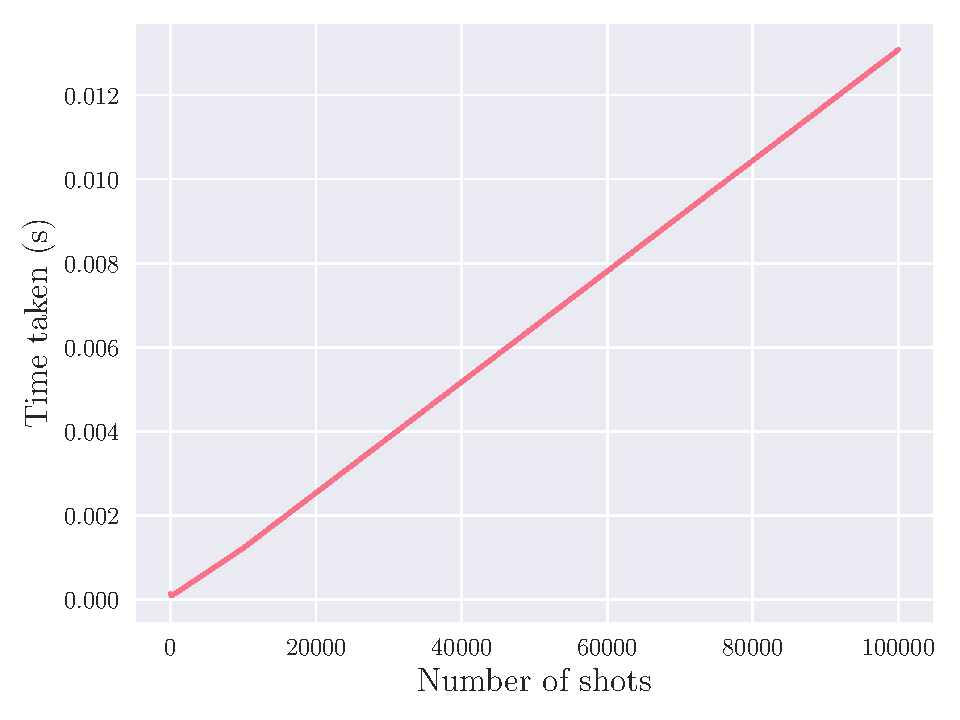
\includegraphics[width=0.7\linewidth]{image/time_vs_shots.pdf}
	\caption{Time taken in seconds for the measurement process as a function of the number of shots.}
	\label{fig:timed_shots}
\end{figure}

The time taken for every measurement with $ 10^5 $ shot is around $ 0.008374 s$. The total time taken for every calculation should also depend on the number of function calls and the length of the qubit Hamiltonian. 



\section{State Initialisation for ADAPT-VQE}
\label{sec:initstate}
According to~\cite{tang2021}, the operator pools $V$ and $G$ should be complete, i.e. any real state $ \ket{\psi} $ can be rotated to another state $ \ket{ \phi} $ with
\begin{equation}
	\ket{\phi} = \prod_{k} e^{\theta V_k} \ket{\psi}.
\end{equation}
However, the ADAPT-VQE stops when the gradient is $ 0 $ or below a certain threshold. Even after removing the even Pauli strings, i.e. Pauli string with an even number of $ Y $ operators, the operator gradient can still vanish for some states $ \ket{\psi}  $. Most noticeably, the $ \ket{0 \ldots 0} $ state. We will provide an example of where all the gradients of the operators vanish, and the ADAPT process stops after one iteration without converging to the correct state. 

For the case of three qubits, the complete $ V $ pool is $ \{ V \} = \{iYZZ, iIYZ, iIIY, iIYI\}$. The term $iYZZ$ can be written in matrix notation as Equation~\eqref{eq:matrixiYZZ}.
\begin{equation}
	\label{eq:matrixiYZZ}
	iYZZ = \begin{pmatrix}
	0 & 0 & 0 & 0 & 1 & 0 & 0 & 0 & \\ 
	0 & 0 & 0 & 0 & 0 & -1 & 0 & 0 & \\ 
	0 & 0 & 0 & 0 & 0 & 0 & -1 & 0 & \\ 
	0 & 0 & 0 & 0 & 0 & 0 & 0 & 1 & \\ 
	-1 & 0 & 0 & 0 & 0 & 0 & 0 & 0 & \\ 
	0 & 1 & 0 & 0 & 0 & 0 & 0 & 0 & \\ 
	0 & 0 & 1 & 0 & 0 & 0 & 0 & 0 & \\ 
	0 & 0 & 0 & -1 & 0 & 0 & 0 & 0 & \\ 
	\end{pmatrix}.
\end{equation}


Initialising the state $\ket{\psi}$
\[ \ket{\psi} = \ket{000}, \] 
for the operator selection process, we then calculate the gradient of each operator in the pool for an arbitrary Hamiltonian with real coefficients, which is true when time-reversal symmetry is preserved. The Hamiltonian of choice is
\begin{equation}
	\label{eq:0gradHamiltonian}
	H = 2IIZ - 0.5IXX + 0.5IYY + 2 ZZI
\end{equation}
in matrix notation that is
\begin{equation}
	\label{eq:0gradHmat}
\begin{pmatrix}
4 & 0 & 0 & -1 & 0 & 0 & 0 & 0  \\
0 & 0 & 0 & 0 & 0 & 0 & 0 & 0  \\
0 & 0 & 0 & 0 & 0 & 0 & 0 & 0  \\
-1 & 0 & 0 & -4 & 0 & 0 & 0 & 0  \\
0 & 0 & 0 & 0 & 0 & 0 & 0 & -1  \\
0 & 0 & 0 & 0 & 0 & -4 & 0 & 0  \\
0 & 0 & 0 & 0 & 0 & 0 & 4 & 0  \\
0 & 0 & 0 & 0 & -1 & 0 & 0 & 0  \\
\end{pmatrix}	
\end{equation}
The gradient is calculated using Equation~\eqref{eq:selection-criteria}. The commutator $ [H,A] $ with $ A=iYZZ $ is then

\begin{align*}
	[H,A] = HA-AH &=
	\begin{pmatrix}
4 & 0 & 0 & -1 & 0 & 0 & 0 & 0  \\
0 & 0 & 0 & 0 & 0 & 0 & 0 & 0  \\
0 & 0 & 0 & 0 & 0 & 0 & 0 & 0  \\
-1 & 0 & 0 & -4 & 0 & 0 & 0 & 0  \\
0 & 0 & 0 & 0 & 0 & 0 & 0 & -1  \\
0 & 0 & 0 & 0 & 0 & -4 & 0 & 0  \\
0 & 0 & 0 & 0 & 0 & 0 & 4 & 0  \\
0 & 0 & 0 & 0 & -1 & 0 & 0 & 0  \\
\end{pmatrix}
\begin{pmatrix}
0 & 0 & 0 & 0 & 1 & 0 & 0 & 0  \\
0 & 0 & 0 & 0 & 0 & -1 & 0 & 0  \\
0 & 0 & 0 & 0 & 0 & 0 & -1 & 0  \\
0 & 0 & 0 & 0 & 0 & 0 & 0 & 1  \\
-1 & 0 & 0 & 0 & 0 & 0 & 0 & 0  \\
0 & 1 & 0 & 0 & 0 & 0 & 0 & 0  \\
0 & 0 & 1 & 0 & 0 & 0 & 0 & 0  \\
0 & 0 & 0 & -1 & 0 & 0 & 0 & 0  \\
\end{pmatrix} \\ 
		      &- \begin{pmatrix}
0 & 0 & 0 & 0 & 1 & 0 & 0 & 0  \\
0 & 0 & 0 & 0 & 0 & -1 & 0 & 0  \\
0 & 0 & 0 & 0 & 0 & 0 & -1 & 0  \\
0 & 0 & 0 & 0 & 0 & 0 & 0 & 1  \\
-1 & 0 & 0 & 0 & 0 & 0 & 0 & 0  \\
0 & 1 & 0 & 0 & 0 & 0 & 0 & 0  \\
0 & 0 & 1 & 0 & 0 & 0 & 0 & 0  \\
0 & 0 & 0 & -1 & 0 & 0 & 0 & 0  \\
\end{pmatrix}
\begin{pmatrix}
4 & 0 & 0 & -1 & 0 & 0 & 0 & 0  \\
0 & 0 & 0 & 0 & 0 & 0 & 0 & 0  \\
0 & 0 & 0 & 0 & 0 & 0 & 0 & 0  \\
-1 & 0 & 0 & -4 & 0 & 0 & 0 & 0  \\
0 & 0 & 0 & 0 & 0 & 0 & 0 & -1  \\
0 & 0 & 0 & 0 & 0 & -4 & 0 & 0  \\
0 & 0 & 0 & 0 & 0 & 0 & 4 & 0  \\
0 & 0 & 0 & 0 & -1 & 0 & 0 & 0  \\
\end{pmatrix} \\
	&= \begin{pmatrix} 
	0 & 0 & 0 & 0 & 4 & 0 & 0 & 0  \\
	0 & 0 & 0 & 0 & 0 & -4 & 0 & 0  \\
	0 & 0 & 0 & 0 & 0 & 0 & 4 & 0  \\
	0 & 0 & 0 & 0 & 0 & 0 & 0 & -4  \\
	4 & 0 & 0 & 0 & 0 & 0 & 0 & 0  \\
	0 & -4 & 0 & 0 & 0 & 0 & 0 & 0  \\
	0 & 0 & 4 & 0 & 0 & 0 & 0 & 0  \\
	0 & 0 & 0 & -4 & 0 & 0 & 0 & 0 
	\end{pmatrix}.
\end{align*}
and 
\begin{align}
	\label{eq:zerograd}
	\braket{\psi|[H,A]|\psi} &= 
	\begin{pmatrix} 1 & 0 & 0 & 0 & 0 & 0 & 0 & 0  \end{pmatrix} 
	\begin{pmatrix} 
	0 & 0 & 0 & 0 & 4 & 0 & 0 & 0  \\
	0 & 0 & 0 & 0 & 0 & -4 & 0 & 0  \\
	0 & 0 & 0 & 0 & 0 & 0 & 4 & 0  \\
	0 & 0 & 0 & 0 & 0 & 0 & 0 & -4  \\
	4 & 0 & 0 & 0 & 0 & 0 & 0 & 0  \\
	0 & -4 & 0 & 0 & 0 & 0 & 0 & 0  \\
	0 & 0 & 4 & 0 & 0 & 0 & 0 & 0  \\
	0 & 0 & 0 & -4 & 0 & 0 & 0 & 0 
	\end{pmatrix}
	\begin{pmatrix} 1 \\ 0 \\ 0 \\ 0 \\ 0 \\ 0 \\ 0 \\ 0 \end{pmatrix}, \\
	&= \begin{pmatrix} 1 & 0 & 0 & 0 & 0 & 0 & 0 & 0 \end{pmatrix} 
	\begin{pmatrix} 0 \\ 0 \\ 0 \\ -1 \\ 4 \\ 0 \\ 0 \\ 0 \end{pmatrix}, \\
		&= 0.
\end{align}

In Appendix~\ref{app:zerograd} we will show that this is true for all the rest of the operators in the pool when the state $ \ket{000}$ is not the ground state for the system given by Equation~\eqref{eq:0gradHamiltonian}. The initialisation of the state is therefore crucial. We found that by starting in the maximally superposed state, $\ket{+}^{\otimes n}$, the gradients of the operators are non-zero, and the system does converge to the ground state eventually. This will therefore be the choice of initial state for the ADAPT-VQE from now on.

\section{Hydrogen Molecule}
\label{sec:hydrogen_result}

While producing results for the hydrogen molecule, we found that initialising the state in the Hartree-Fock state ($ \ket{1100} $in this case) results in the $ 0 $ gradient problem as described in Section~\ref{sec:initstate} and Appendix~\ref{app:zerograd}. Indeed, all terms of the qubit Hamiltonian shown in Table~\ref{tab:qubit-hamiltonian-h2} do not contribute to the gradient when the state is in the $ \ket{1100} $ or the $ \ket{0000} $ state. 

The qubit Hamiltonian contains $ 15 $ terms. The expected error for $ 10^5 $ shots is $ 0.00316 $. The expected error for the hydrogen molecule is therefore $ 0.012 $. 


\subsection{Exact Energy Simulation}
\begin{figure}[ht]
    \centering
    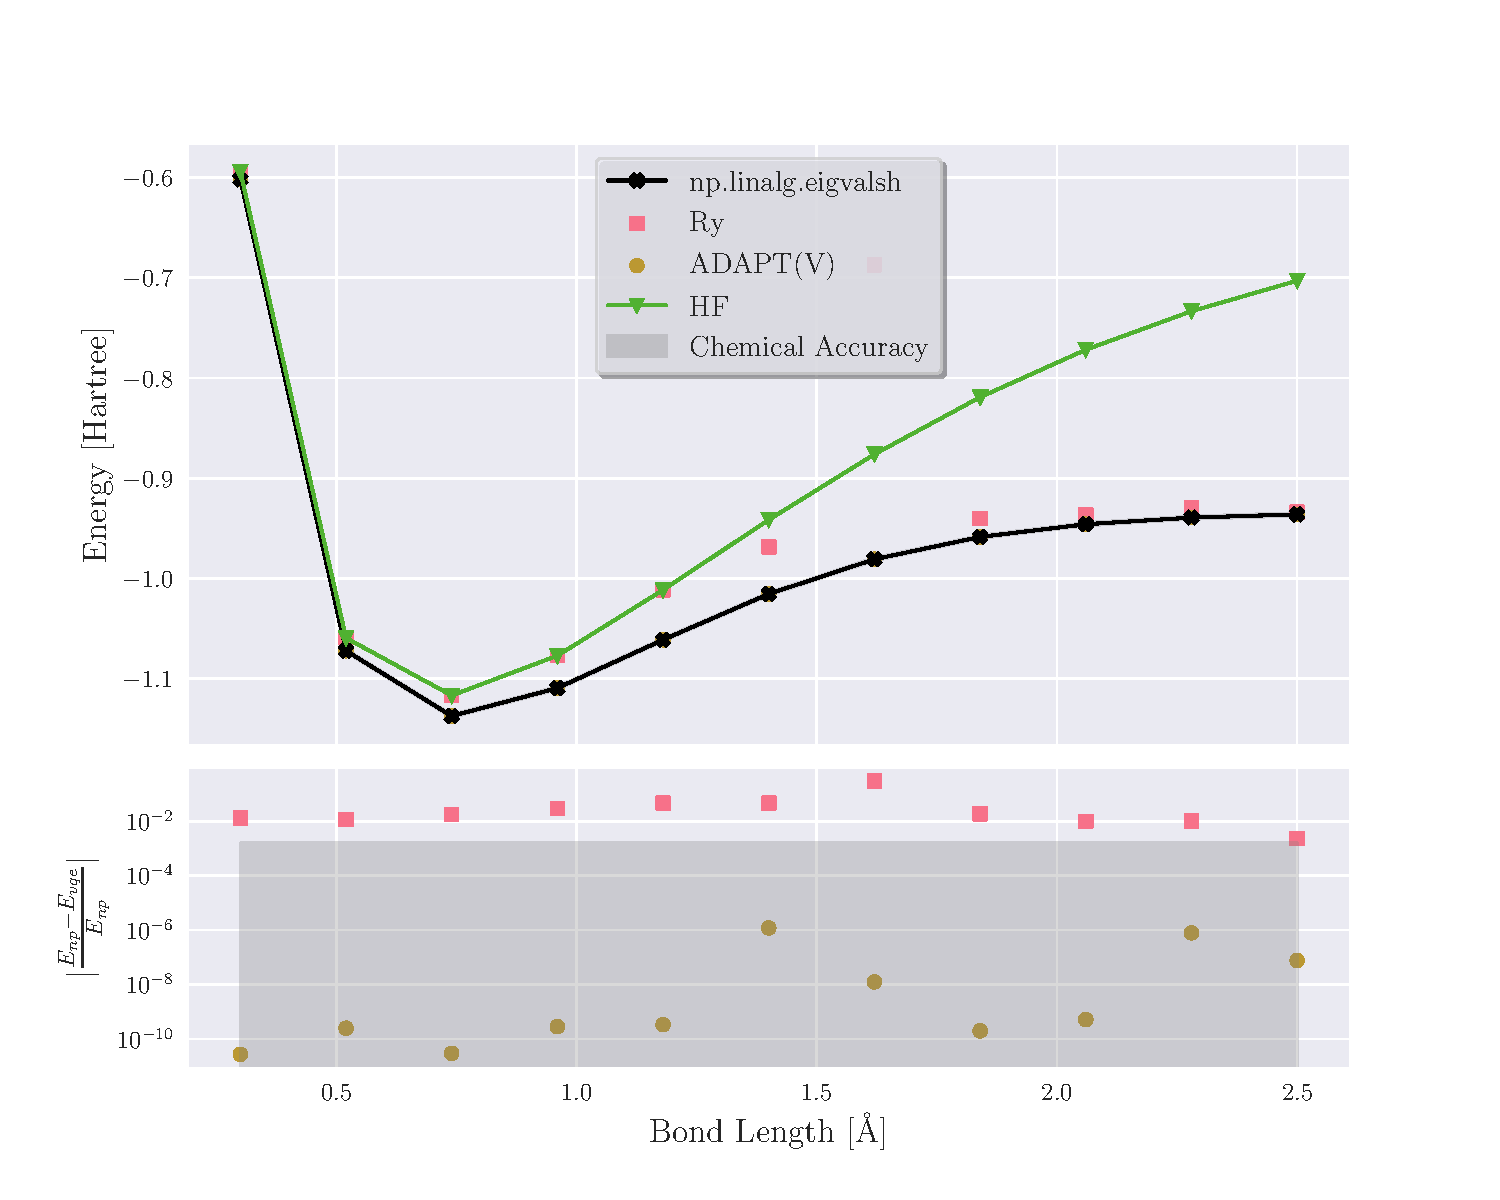
\includegraphics[width=\linewidth]{image/h2_result/nsn/best-nsn.pdf}
    \caption{The Hydrogen molecule with \textbf{exact energy simulation}, showing the comparison between VQE with $ 3 $ repetition and ADAPT-VQE with the $ V $ pool and maximum $ 30 $ ADAPT iterations. Both are minimised using the \texttt{BFGS} method. The VQE was initialised in the HF state and the ADAPT-VQE was initialised in a random real state. The yellow markers are hard to see on the upper plot as they are almost perfectly aligned with the numerical diagonalisation.}
    \label{fig:h2main-nsn}
\end{figure}

We see for the exact energy simulation that the ADAPT-VQE outperforms the VQE and Hartree-Fock by a large margin, and was able to converge to the exact diagonalisation result with an error within orders of $ 10^{-6} $ for both small and large bond length, also achieving chemical accuracy. The Ry ansatz was not able to converge to the true ground state for a small bond length, rather it converges to the HF state. This might be related to the Hartree-Fock initialisation. For large bond lengths where the Hartree-Fock energy is a poor estimation of the ground state, both VQEs exhibit better results than the Hartree-Fock energy. We also note that the performance of the ADAPT-VQE is not affected by the bond length as the error stays the same, suggesting that the qubit-ADAPT ansatz is exact and can represent the ground state with different interactions.


\subsection{Ideal Simulation}
\begin{figure}[ht]
    \centering
    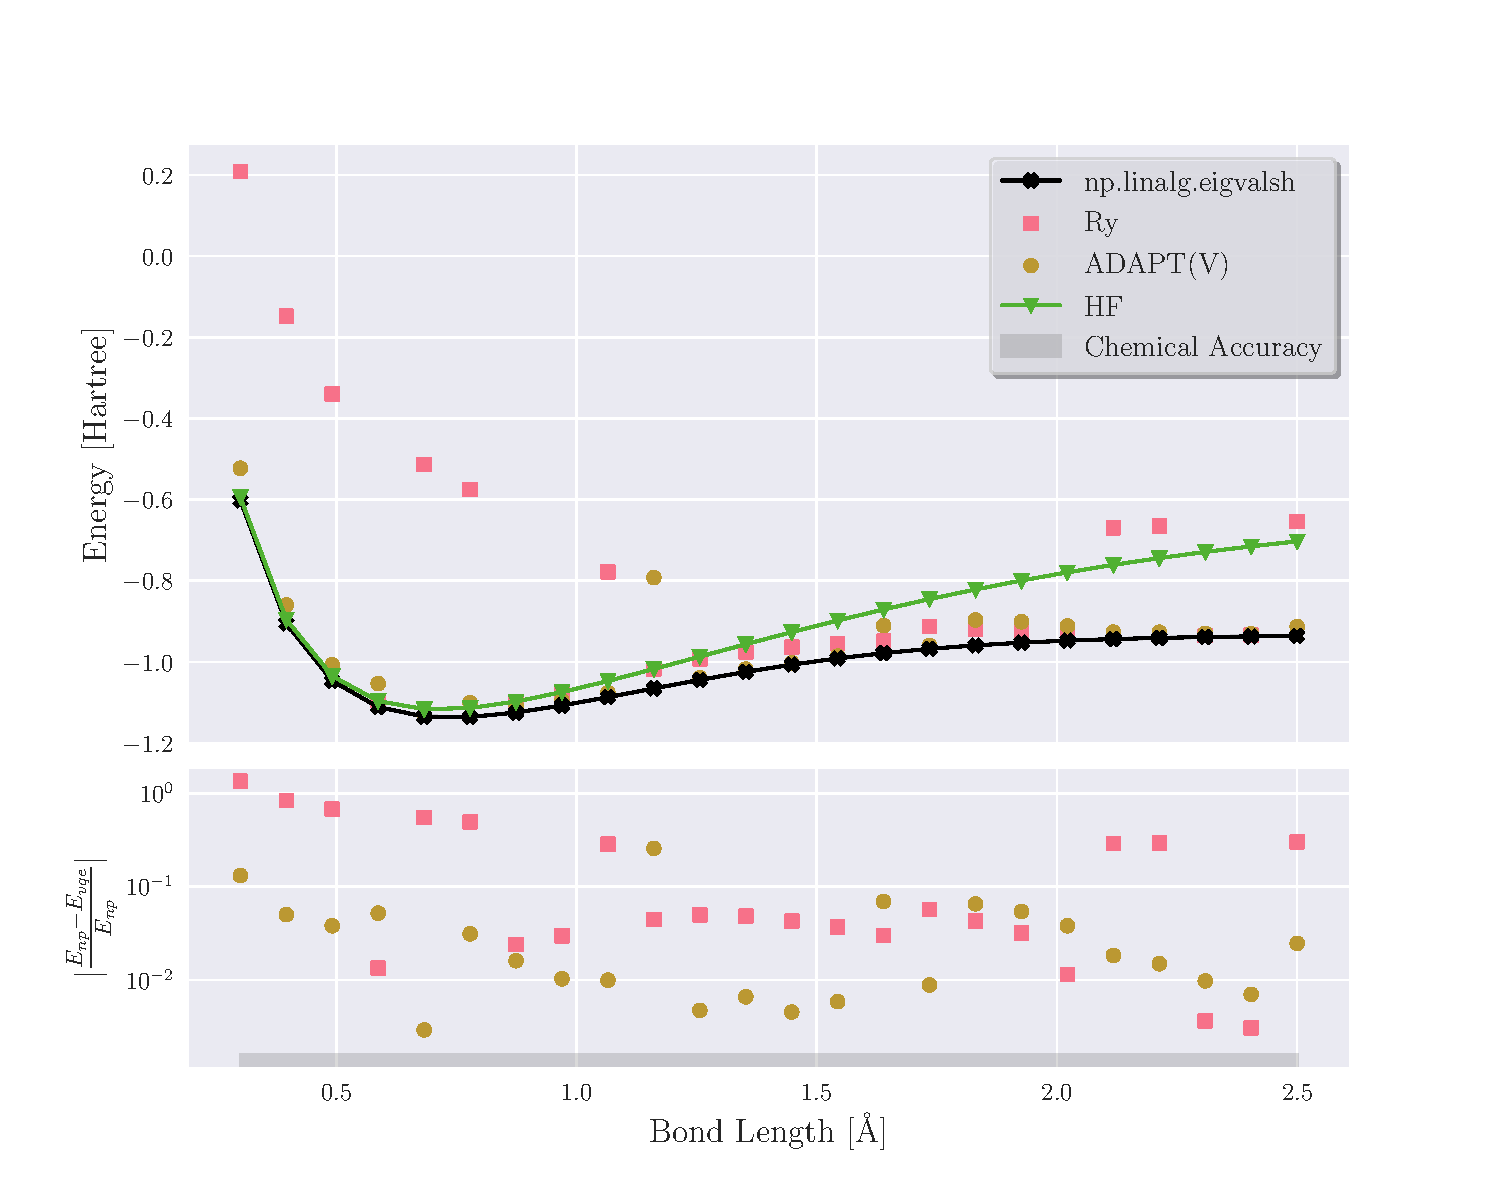
\includegraphics[width=\linewidth]{image/h2_result/simulation/best_sim.pdf}
    \caption{The hydrogen molecule with \textbf{ideal simulation} with $ 100000 $ shots for a maximum of $ 30 $ ADAPT iterations. The ADAPT-VQEs were optimised with the \texttt{COBYLA} method and the VQE with the \texttt{Powell} method. The exponential was decomposed using the \textbf{inverted Staircase} algorithm.}
    \label{fig:h2main-noisy}
\end{figure}

Figure~\ref{fig:h2main-noisy} shows the results for an ideal simulation. Again, ADAPT outperformed the VQE but the results for both were underwhelming and were not chemically accurate. It is still obvious that the ADAPT-VQE is more consistent in terms of performance when it comes to bond length, and the normal VQE with Ry ansatz performs poorly for both low and high bond lengths. Compared with the expected error with this shot noise $ 0.012 $, only a few points between $ 1 - 1.5 \text{Å} $ with the use of the ADAPT-VQE were able to obtain errors of the same magnitude.
The simple shot noise affects the convergence of the ADAPT-VQE greatly. Even with the ADAPT gradient being calculated analytically, the impact of the shot noise is still significant. We hypothesise that the optimisation for the VQE subroutine at every ADAPT iteration might not always converge, causing the state to be in a different state than the state with the optimal parameters for the current iteration. One suggestion to improve the result is to group commuting operators to be measured together to reduce the number of state preparations required.

To test our hypothesis, we ran the system with the same parameters except increasing the maximum iteration to $ 60 $. The result for this is shown in Figure~\ref{fig:60iterh2}. While this did not improve our results it helps us understand the problem better. For all the values, the energy was decreasing with every iteration initially but stopped after $ 10 $ iterations. For the case of $ 0.3 \text{Å} $, the error is below the expected error for the number of shots we use, as we can see from the fluctuation of the error after the convergence. For other bond lengths, however, the results were not able to reach the exact ground state as while more operators were being appended, the error was not decreasing to below the expected error. Meanwhile, the gradient is not small enough for the ADAPT-VQE to stop, which may suggest that with shot noise, the operator gradient might have trouble selecting the operator which changes the state the most. This also tells us that using the expected error is a good metric to evaluate the performance of an ideal simulation. This, incidentally, also results in a large increase of function calls, approximately $ 15000 $, where $ \sim 1000 $ function calls were made for the $ 15 $ iteration case and $ \sim 5000 $ for the $ 30 $ iteration case. This is a sign that the optimisers struggle as the number of parameters increases, which is unsurprising. 

\section{Lipkin-Meshkov-Glick Model}
\label{sec:LMG_result}
Here we showcase results obtained from both exact energy and ideal simulation for the LMG model, for both the $ J=1 $ and $ J=2 $ cases. We will assume $ W=0 $ throughout this section. 

The rewritten and Pauli decomposed Hamiltonian for $ J=1 $ has four terms, and $ J=2 $ has $ 16 $ terms. The expected error for these cases with $ 10^5 $ shots are $ 0.006 $ and $ 0.013 $ respectively. 


\subsection{Exact Energy Simulation}
Figure~\ref{fig:j1main-nsn} and Figure~\ref{fig:j2main-nsn} show the comparison between VQE and ADAPT-VQE for the LMG model with $ J=1 $ and $ J=2 $ for the \textbf{exact energy simulation}, respectively. We found that with $ repetition=1 $, the VQE algorithm was able to converge, but an attempt to improve the result further by adding another layer of gates caused the algorithm to fail to converge completely for the case of rewritten Hamiltonian as shown in Figure~\ref{fig:2repnotok}. For $ J=1 $, apart from a few points where one method did not converge, the convergence was decent for all the methods, with errors in orders of $ 10^{-8} $.  For the $ J=2 $ case the ADAPT with Pauli decomposed energy produced the best results with errors orders of $ 10^{-8} $ while other methods had errors between $ 10^{-2} $ and $ 10^{-1} $. In both cases, the ADAPT performed better than the VQE respectively by being more stable for all interaction strength and lower error. 

\begin{figure}[ht]
	\centering
	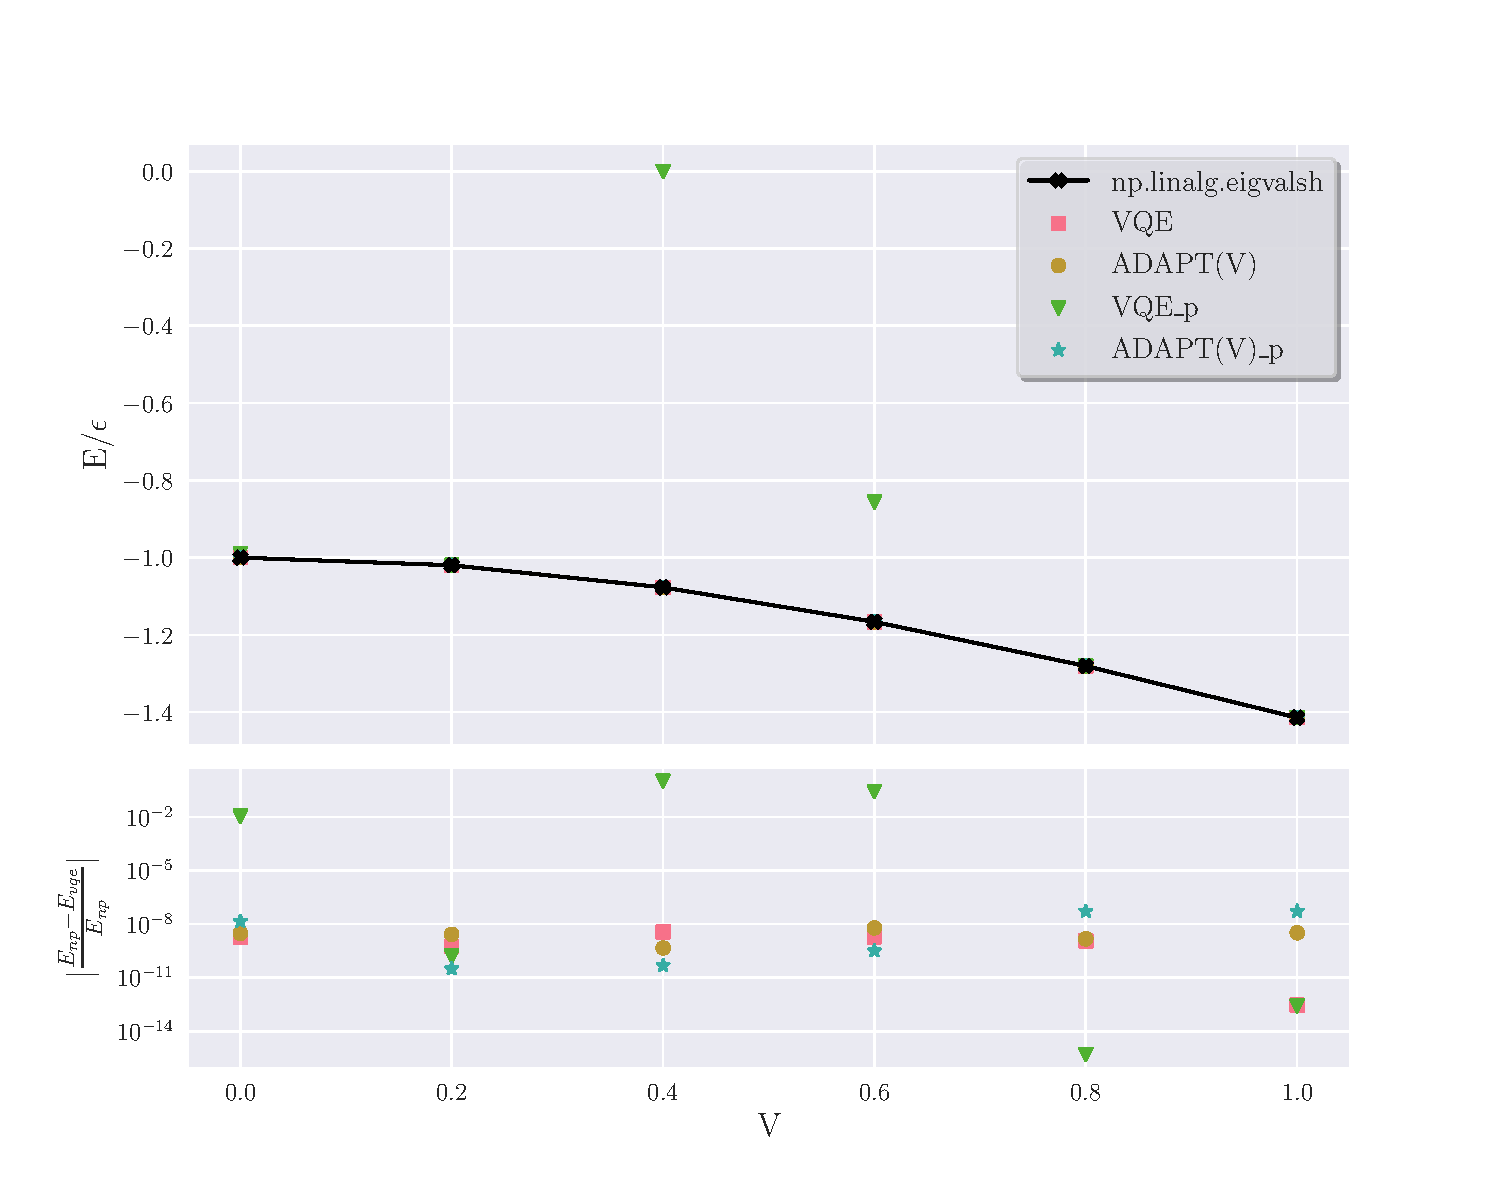
\includegraphics[width=\linewidth]{image/lipkin_result/j1main_False.pdf}
	\caption{The LMG model with $ J=1 $ with \textbf{exact energy simulation}, showing the comparison between VQE with $ 1 $ repetition and ADAPT-VQE with the $ V $  pool and maximum $ 12 $ ADAPT iterations. The label with \textit{\_p} means that the Hamiltonian was mapped using Pauli decomposition, otherwise, Equation~\eqref{eq:rewrite} was used. Both were optimised with \texttt{BFGS} method.}
	\label{fig:j1main-nsn}
\end{figure}

\begin{figure}[ht]
	\centering
	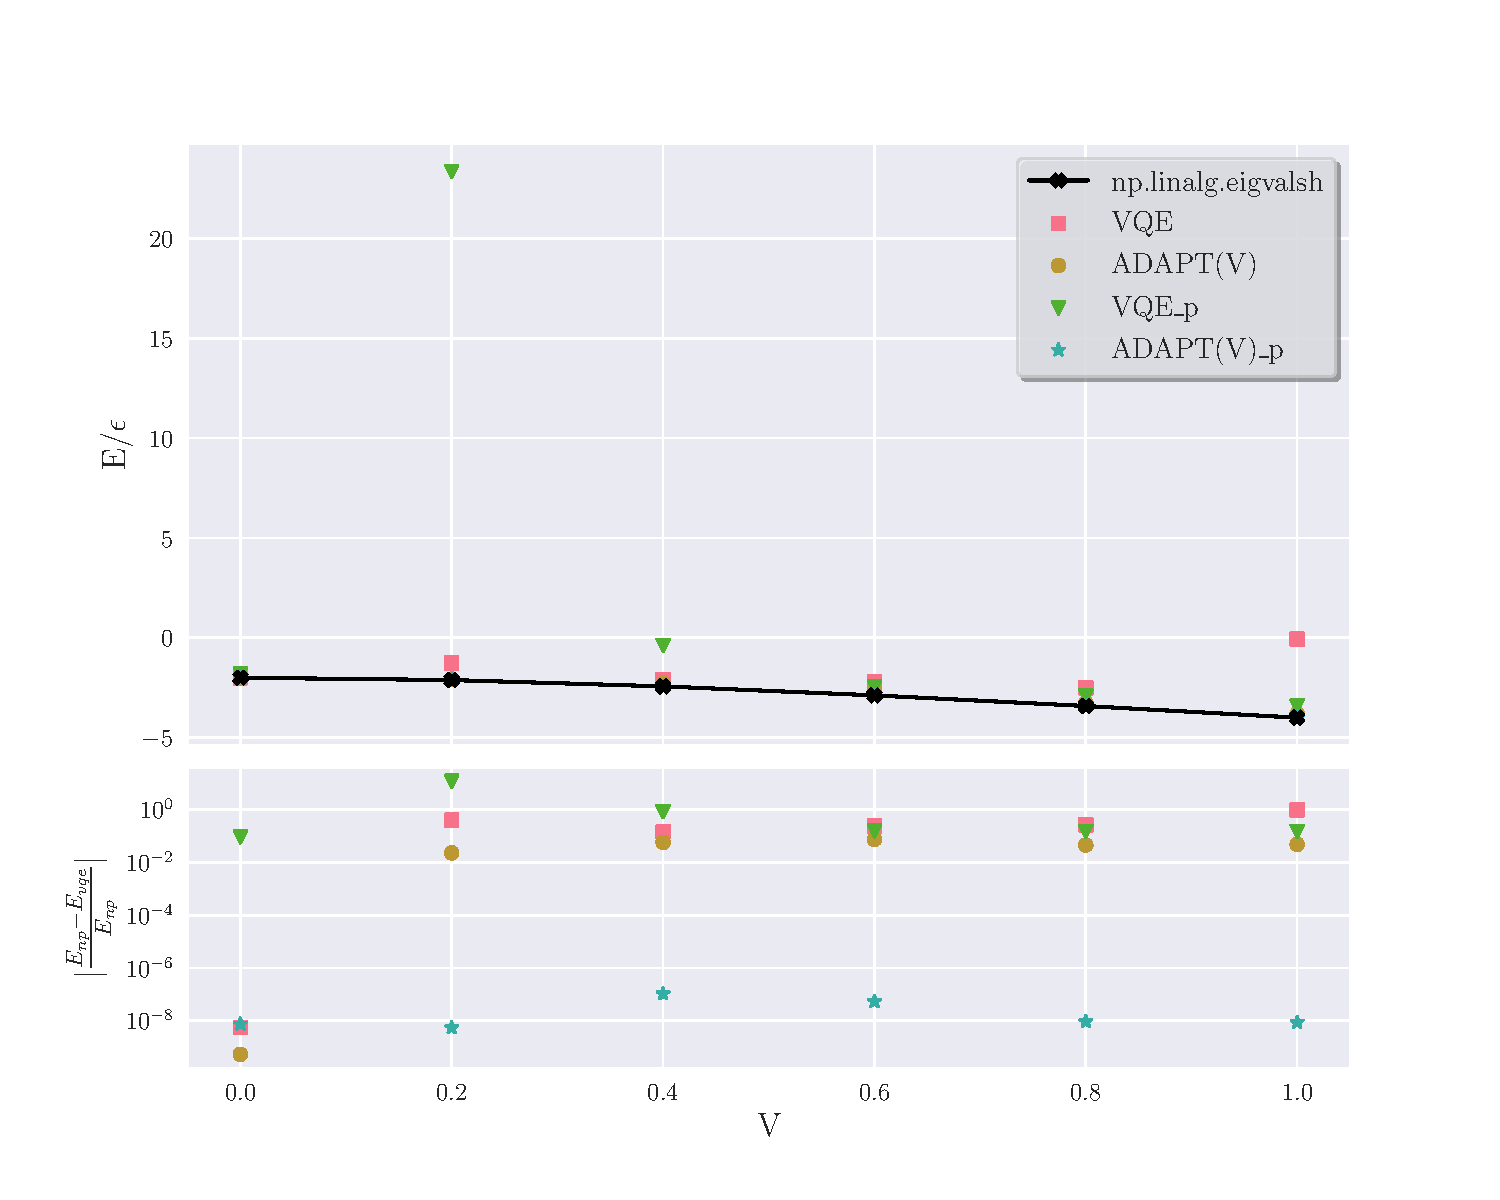
\includegraphics[width=\linewidth]{image/j2main_False.pdf}
	\caption{The LMG model with $ J=2 $ with \textbf{exact energy simulation}, showing the comparison between VQE with $ 1 $ repetition and ADAPT-VQE with the $ V $  pool and maximum $ 12 $ ADAPT iterations. Both were optimised with \texttt{BFGS} method. The label with \textit{\_p} means that the Hamiltonian was mapped using Pauli decomposition, otherwise, Equation~\eqref{eq:rewrite} was used.}
	\label{fig:j2main-nsn}
\end{figure}


\subsection{Ideal Simulation}
Figures~\ref{fig:j1main-noisy} and~\ref{fig:j2main-noisy} show the results for ideal simulations again for both $ J=1,2 $ as well as both mapping.
\begin{figure}[ht]
    \centering
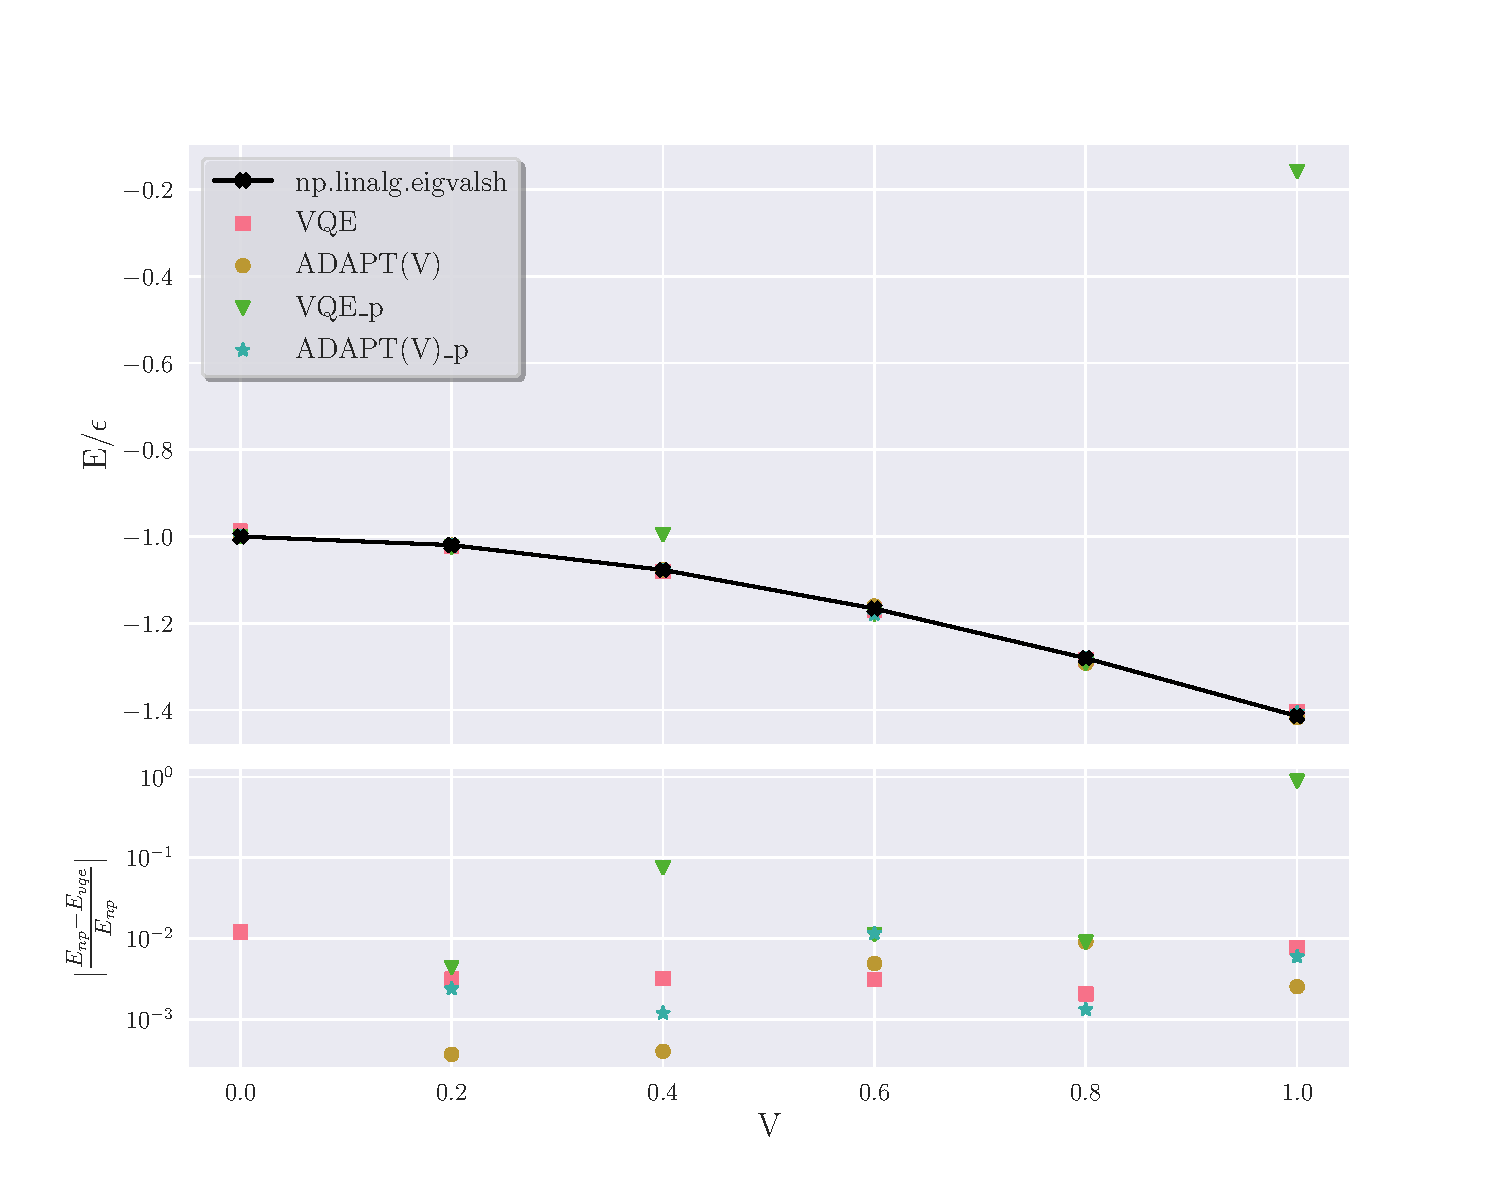
\includegraphics[width=\linewidth]{image/lipkin_result/j1main_True.pdf}
    \caption{The LMG model with $ J=1 $ with \textbf{ideal simulation}, showing the comparison between VQE with $ 1 $ repetition and ADAPT-VQE with the $ V $  pool and $ G $ pool and maximum $ 12 $ ADAPT iterations. The ADAPT-VQE was optimised with the \texttt{COBYLA} method and the normal VQE was with \texttt{Powell}. The label with \textit{\_p} means that the Hamiltonian was mapped using Pauli decomposition, otherwise, Equation~\eqref{eq:rewrite} was used.}
    \label{fig:j1main-noisy}
\end{figure}


\begin{figure}[ht]
    \centering
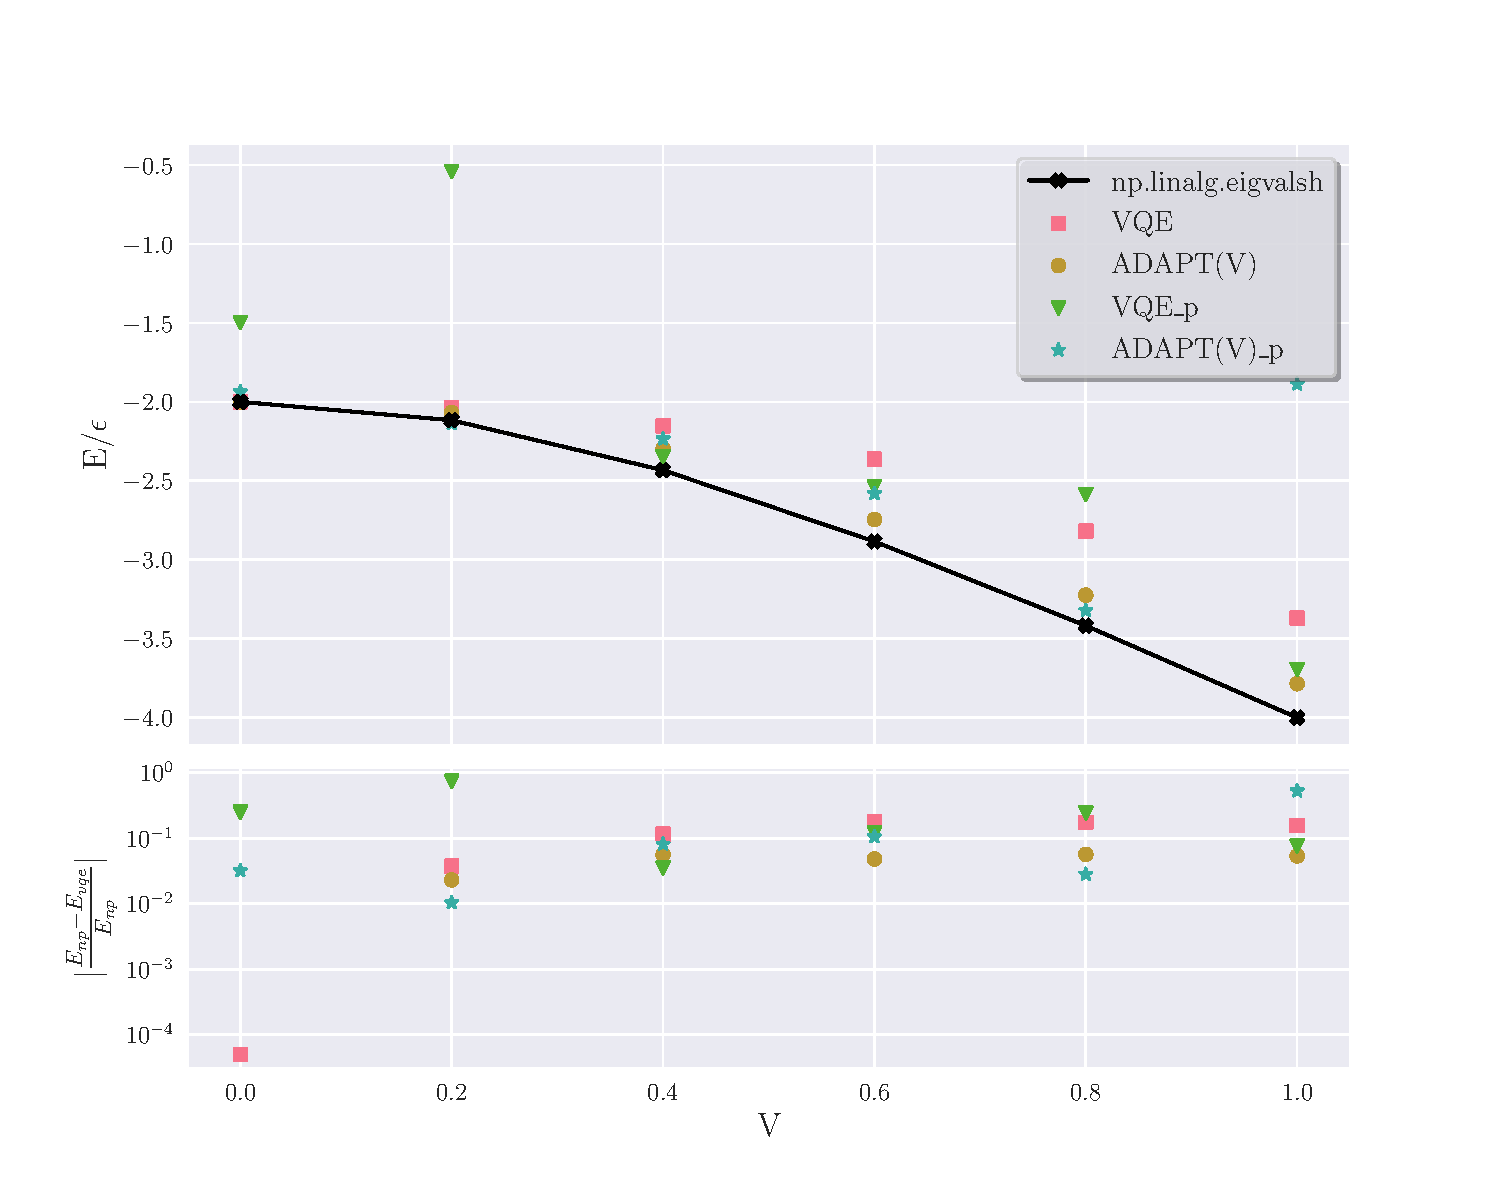
\includegraphics[width=\linewidth]{image/lipkin_result/j2main_True.pdf}
    \caption{The LMG model with $ J=2 $ with \textbf{ideal simulation}, showing the comparison between VQE with $ 1 $ repetition and ADAPT-VQE with the $ G $  pool and $ V $  pool and maximum $ 12 $ ADAPT iterations. The ADAPT-VQE was optimised with the \texttt{COBYLA} method and the normal VQE was with \texttt{Powell}. The label with \textit{\_p} means that the Hamiltonian was mapped using Pauli decomposition, otherwise, Equation~\eqref{eq:rewrite} was used.}
    \label{fig:j2main-noisy}
\end{figure}




\subsection{Circuit Properties}
\label{sub:CircuitProperties}

\begin{table}[ht]
	\centering
	\caption{Table comparison between the fixed-form ansatz and the ADAPT-VQE for both Hamiltonians for the $ J=2 $ case with $ V=1 $ .}
	\label{tab:circuit_prop}

	\begin{tabular}{c c c c c}
		\toprule
		& \textbf{Parameters} &\textbf{Gates} & \textbf{CNOT gates} & \textbf{Energy Function Evaluation} \\
		\midrule

	    Hardware Efficient & 8 & 11 & 3 & 1654\\
		qubit-ADAPT & 12 & 128 & 46 & 846 \\
		Hardware Efficient (Pauli) & 6 & 8 & 2 & 549 \\
		qubit-ADAPT (Pauli) & 12 & 66 & 14 & 801 \\
		\bottomrule
		
	\end{tabular}
\end{table}

Table~\ref{tab:circuit_prop} shows the comparison between the fixed-form ansatzes and the qubit-ADAPTs for the $ J=1 $ case with $ V=1 $. Both qubit-ADAPTs have more parameters and gates, but the number of energy function evaluations is also less for qubit-ADAPT than the HardwareEfficientAnsatz. Pauli-decomposing the Hamiltonian also reduces the resources required to solve the problem. As the hardware efficient ansatz has much fewer gates and CNOT gates, it is expected that there are limitations to the expressibility of the ansatz, hence higher error.

\subsection{Optimisation Methods Comparison}
\label{sub:Optimisers}
In this subsection, we will delve into an analysis of the optimisers used for the VQE and ADAPT-VQE. All optimisers were capped at $ 10000 $ maximum iterations, which is usually never reached. We will choose the best optimisers for both the fixed-form ansatz and the ADAPT-VQE for the main results depending on whether shot noise is present or not.

\subsubsection{Best Optimisers for Fixed-Form Ansatz }%
\label{ssub:BestOptimisersforHW}
This is tested using the qubit Hamiltonian from Equation~\eqref{eq:qubit-hamiltonian-j1-rewrite} and ~\eqref{eq:qubit-hamiltonian-j2-rewrite}  for both the $ J=1 $ and $ J=2 $ cases, which was mapped to a $ 1 $ and $ 2 $ qubits Hamiltonian respectively.

\paragraph{Exact Energy Simulation}
Figure~\ref{fig:opt-fixed-form} shows the comparison between different optimisers for the fixed-form ansatz with \texttt{Rx} and \texttt{Ry} gates without shot noise.

\begin{figure}[ht]
    \centering
    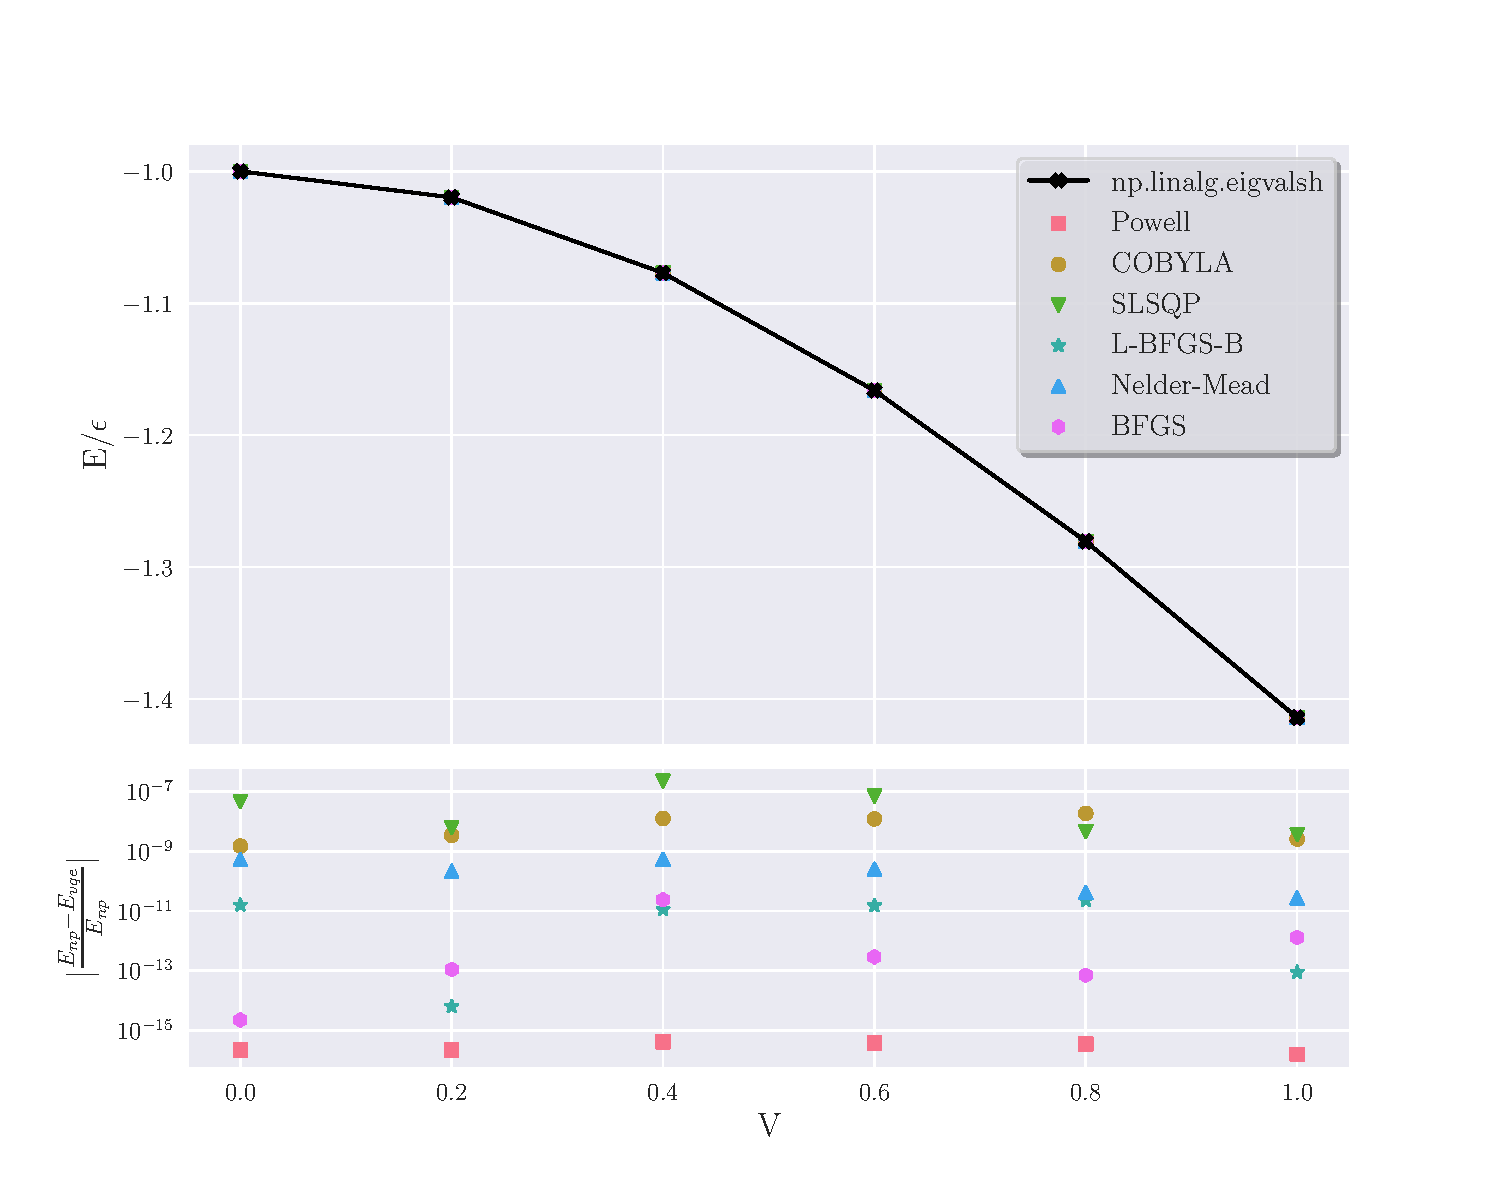
\includegraphics[width=0.45\linewidth]{image/lipkin_result/vqe-opt/cmp_opt_vqe_p_J=1.pdf }
    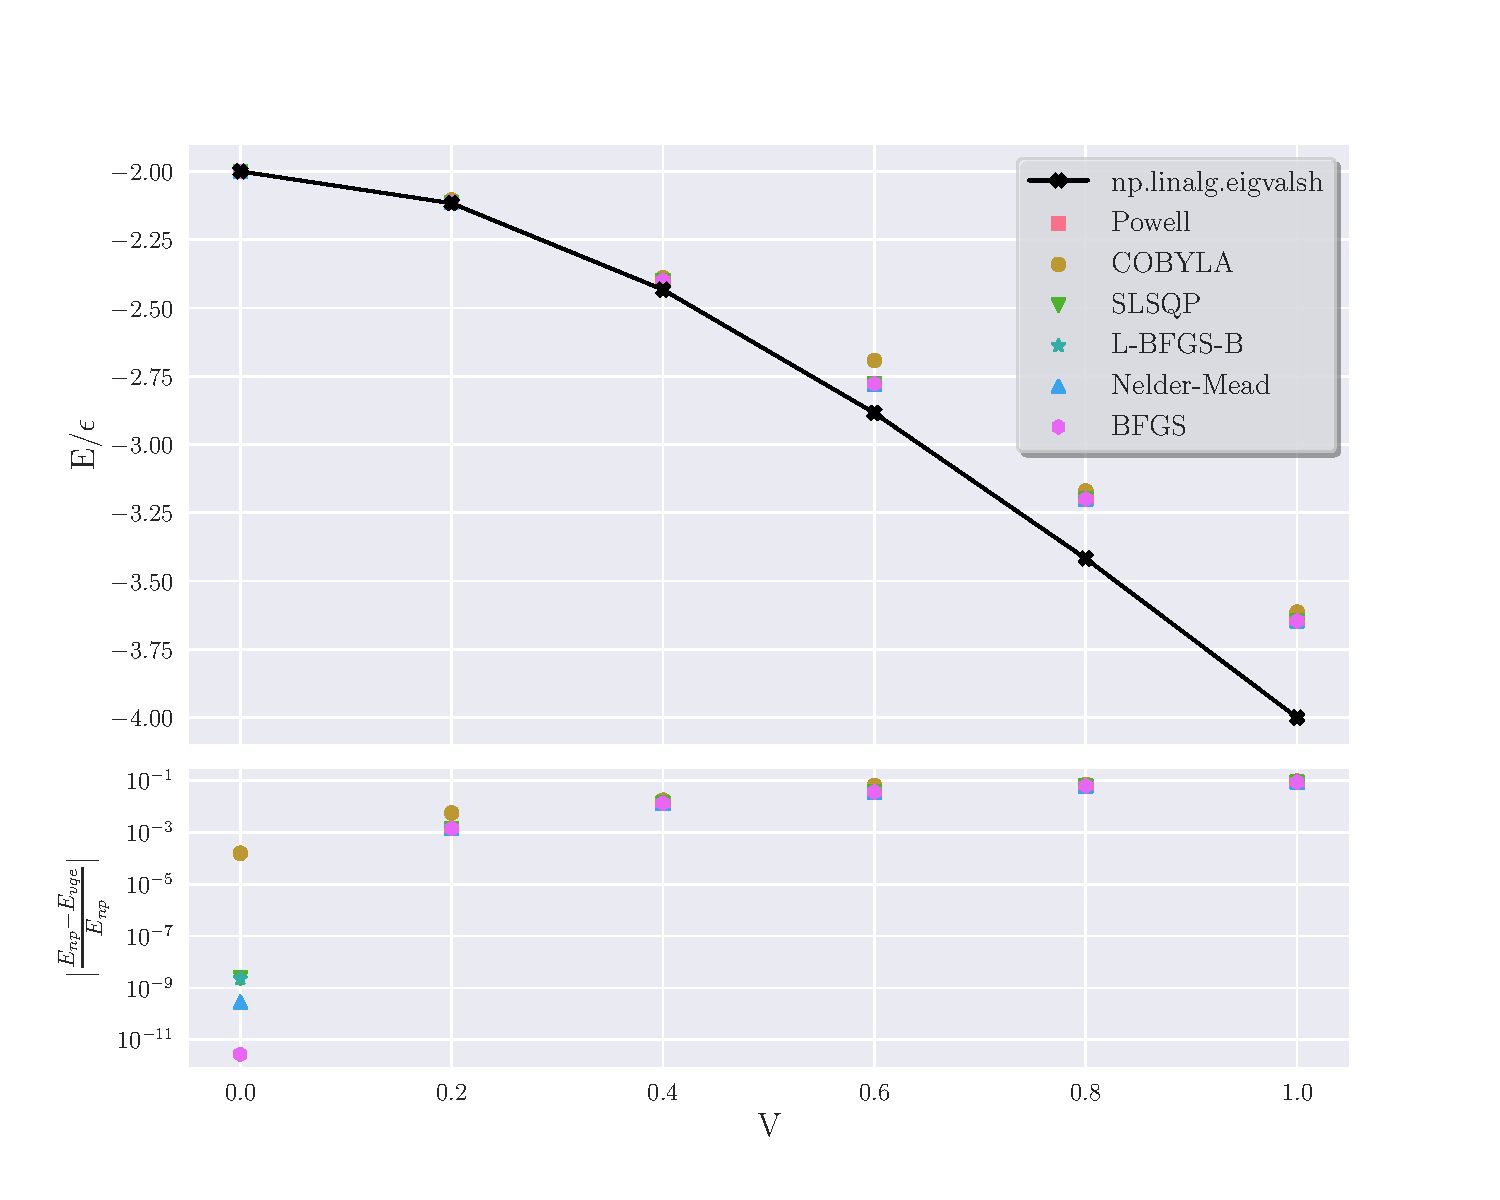
\includegraphics[width=0.45\linewidth]{image/lipkin_result/vqe-opt/cmp_opt_vqe_p_J=2.pdf }
    \caption{Comparison amongst different optimisers for the fixed-form ansatz with \textbf{ exact energy simulation } for $ J=1 $ and $ 2 $  .}
    \label{fig:opt-fixed-form}
\end{figure}

The $ J=1 $ case suggests that Powell is able to achieve the lowest error and the $ J=2 $ case suggests the same, for where the ansatz is expressive enough. Therefore the \texttt{Powell} method will be the choice of optimiser for the fixed-form ansatz for the main exact energy results.

\paragraph{Ideal Simulation}
\begin{figure}[ht]
	\centering
	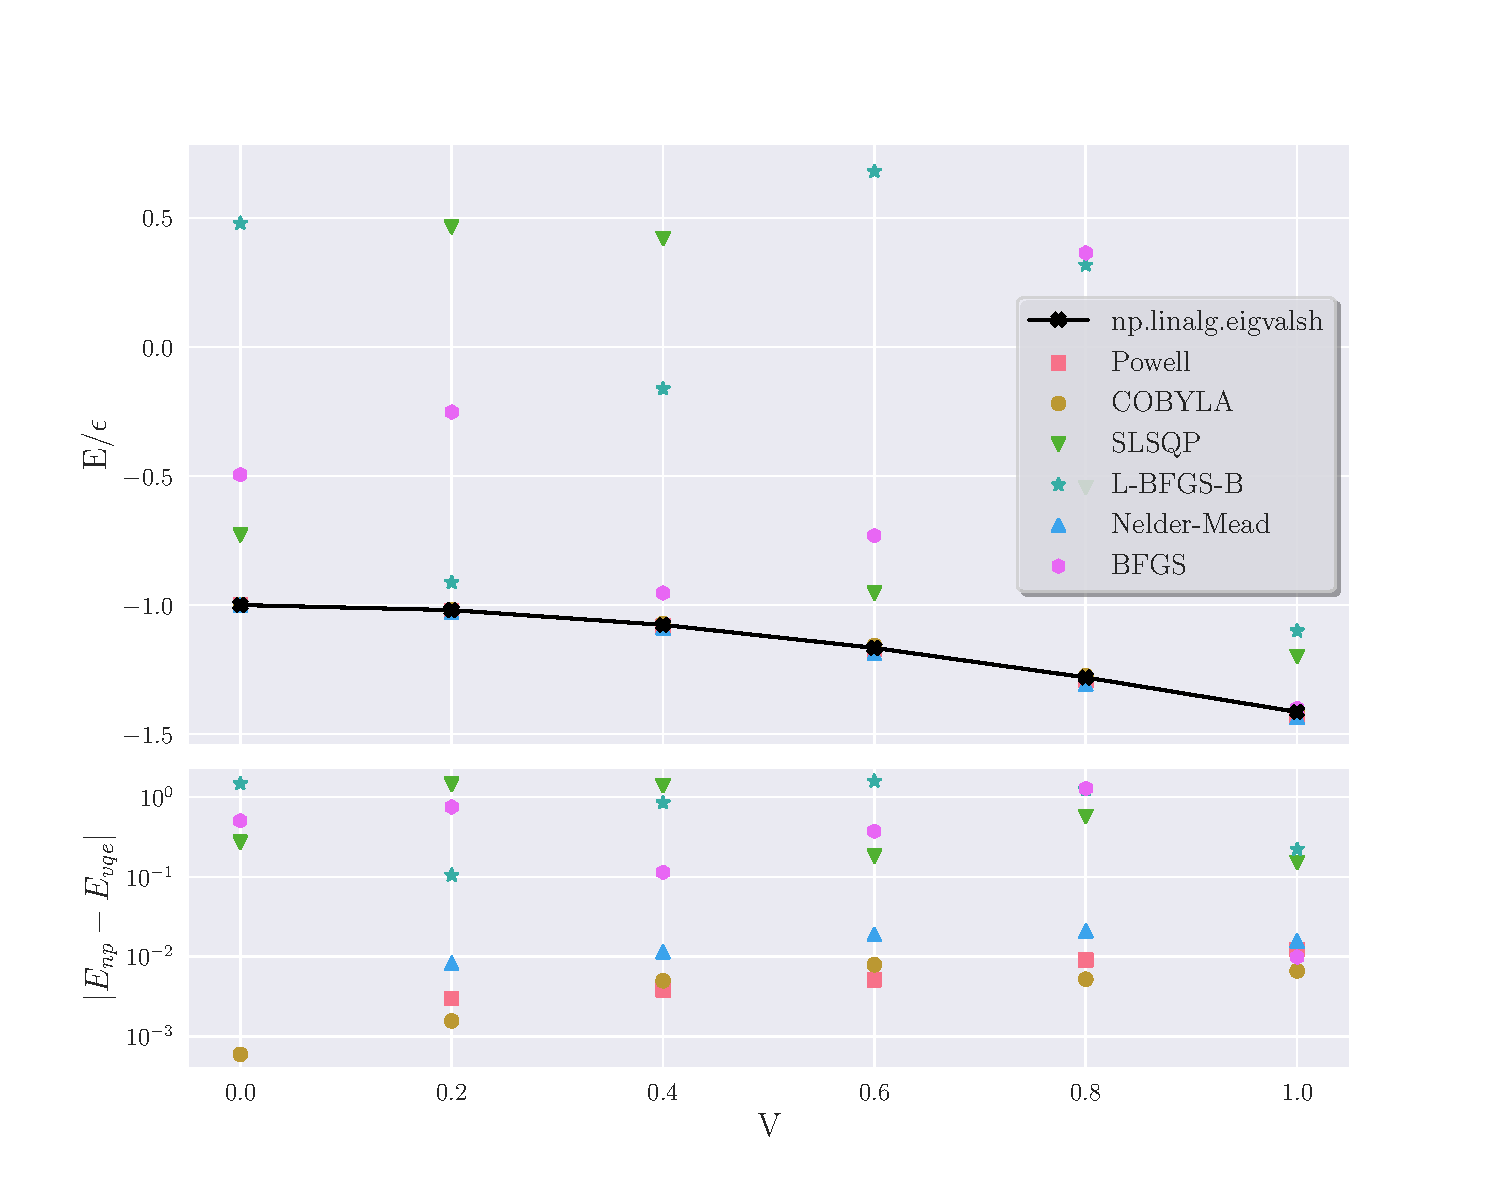
\includegraphics[width=0.45\linewidth]{image/lipkin_result/vqe-opt/cmp_opt_vqe_p_ee100000_J=1.pdf}
	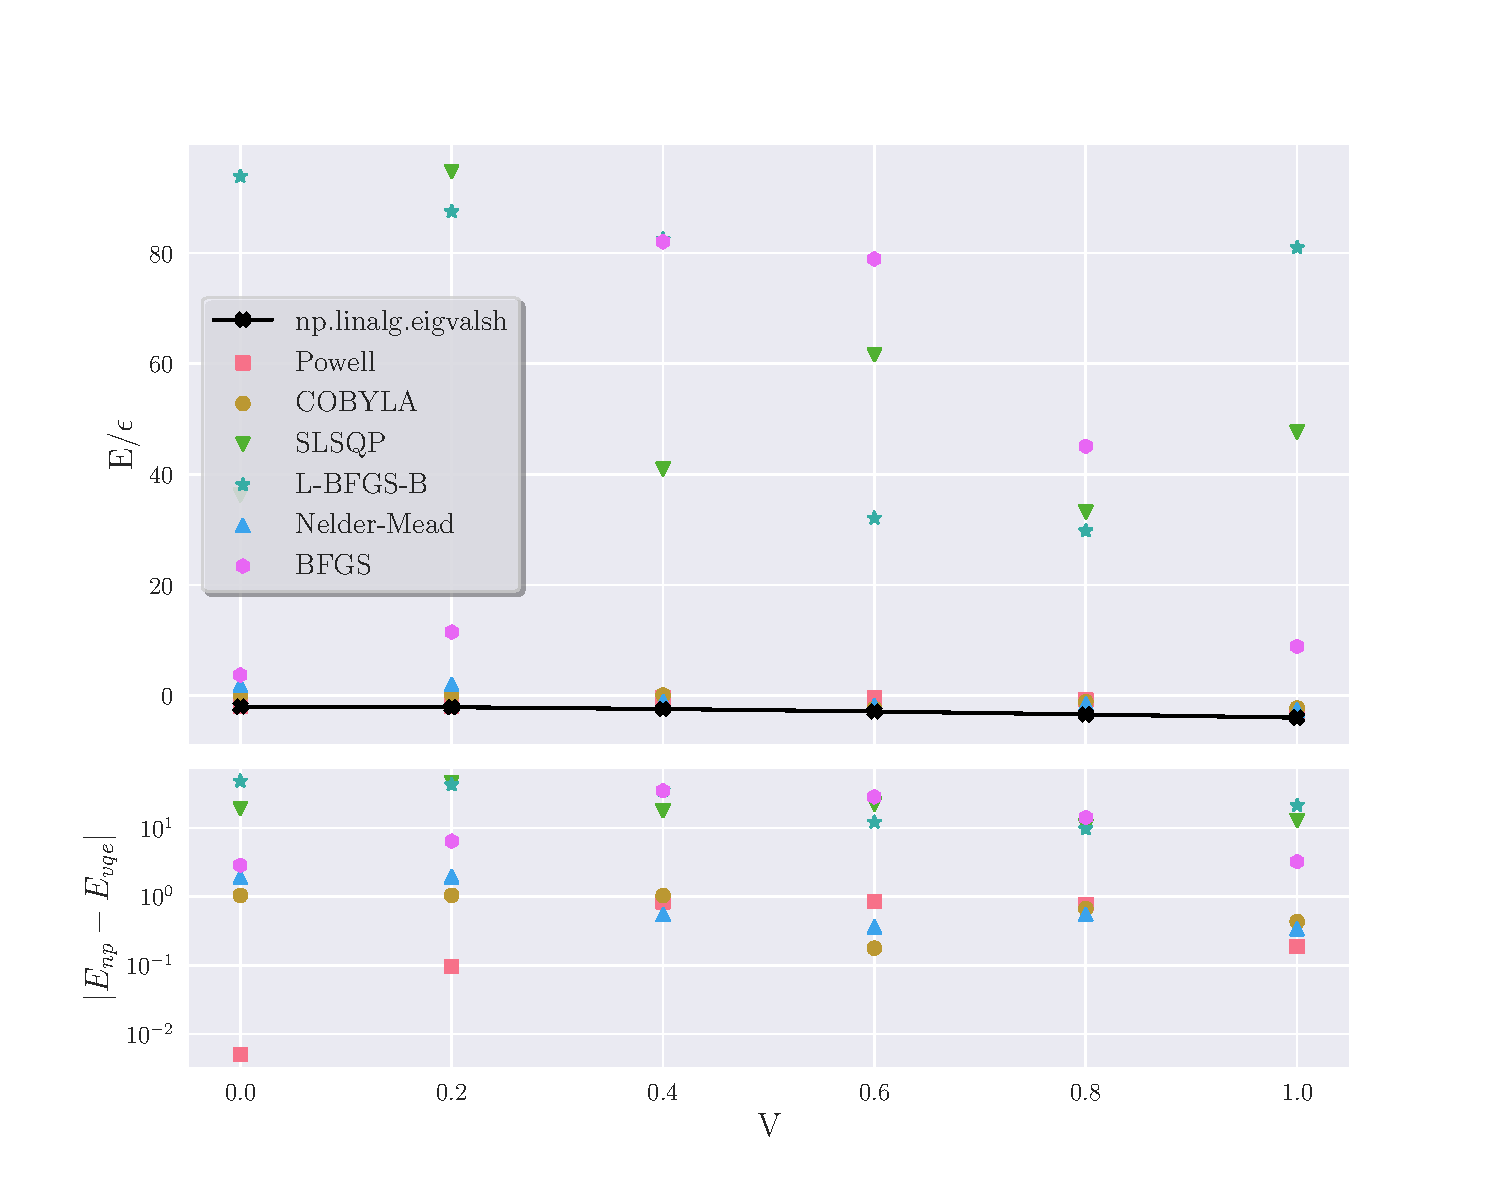
\includegraphics[width=0.45\linewidth]{image/lipkin_result/vqe-opt/cmp_opt_vqe_p_ee100000_J=2.pdf}
	\caption{Comparison amongst different optimisers for the fixed-form ansatz with $ 100000 $ shots for $ J=1$ (left) $J=2 $ (right).}
	\label{fig:Opt-fixed-form-noisy}
\end{figure}

Figure~\ref{fig:Opt-fixed-form-noisy} shows the comparison between different optimisers for the fixed-form ansatz with shot noise. The most robust optimisers for the fixed-form ansatz with shot noise are \texttt{COBYLA} and \texttt{Powell}. The \texttt{Nelder-Mead} method produced reasonable results for some interaction strength but struggles at large interaction strength. Since Powell has better performance for both cases, it will be the choice of optimiser for the main results.

\subsubsection{Best Optimisers for the qubit-ADAPT-VQE}%
\label{ssub:BestOptimisersforADAPT}

\paragraph{Exact Energy Simulation}
Figure~\ref{fig:OptAdapt} shows the comparison between different optimisers for the ADAPT-VQE without shot noise. We see that BFGS and L-BFGS-B were able to achieve the lowest energy errors.
\begin{figure}[ht]
	\centering
	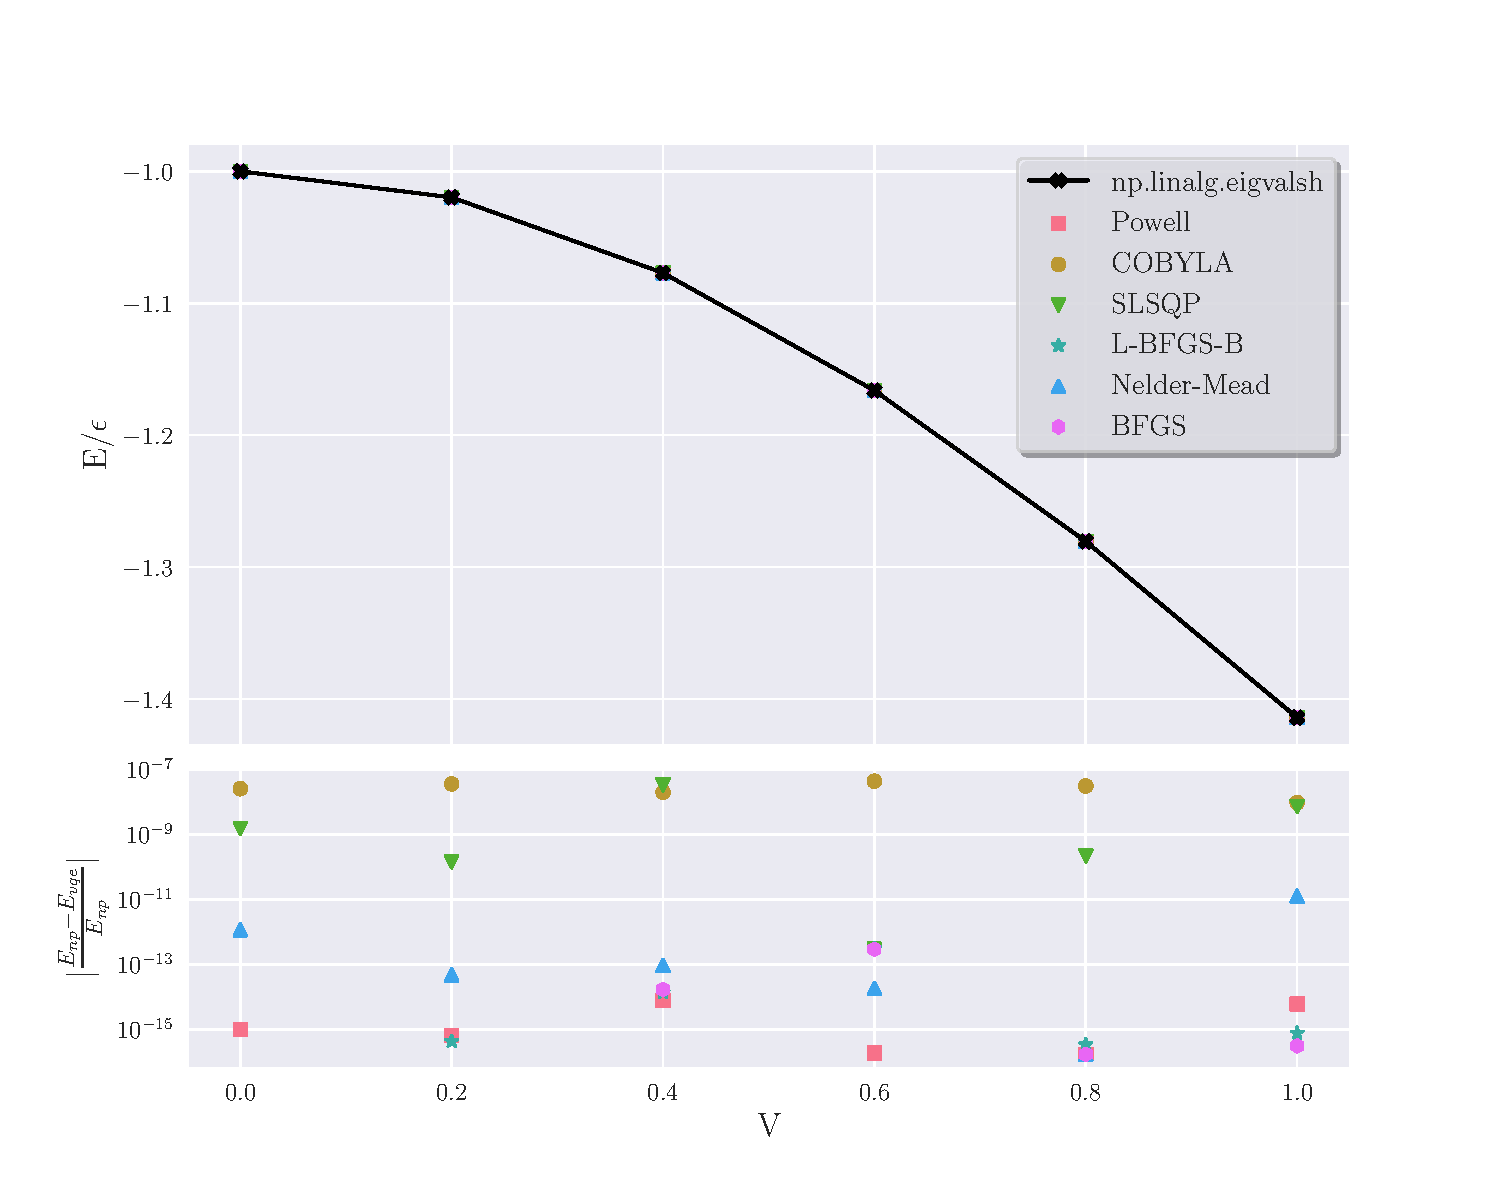
\includegraphics[width=0.47\linewidth]{image/lipkin_result/adapt-opt/cmp_opt_adapt_p_J=1.pdf}
	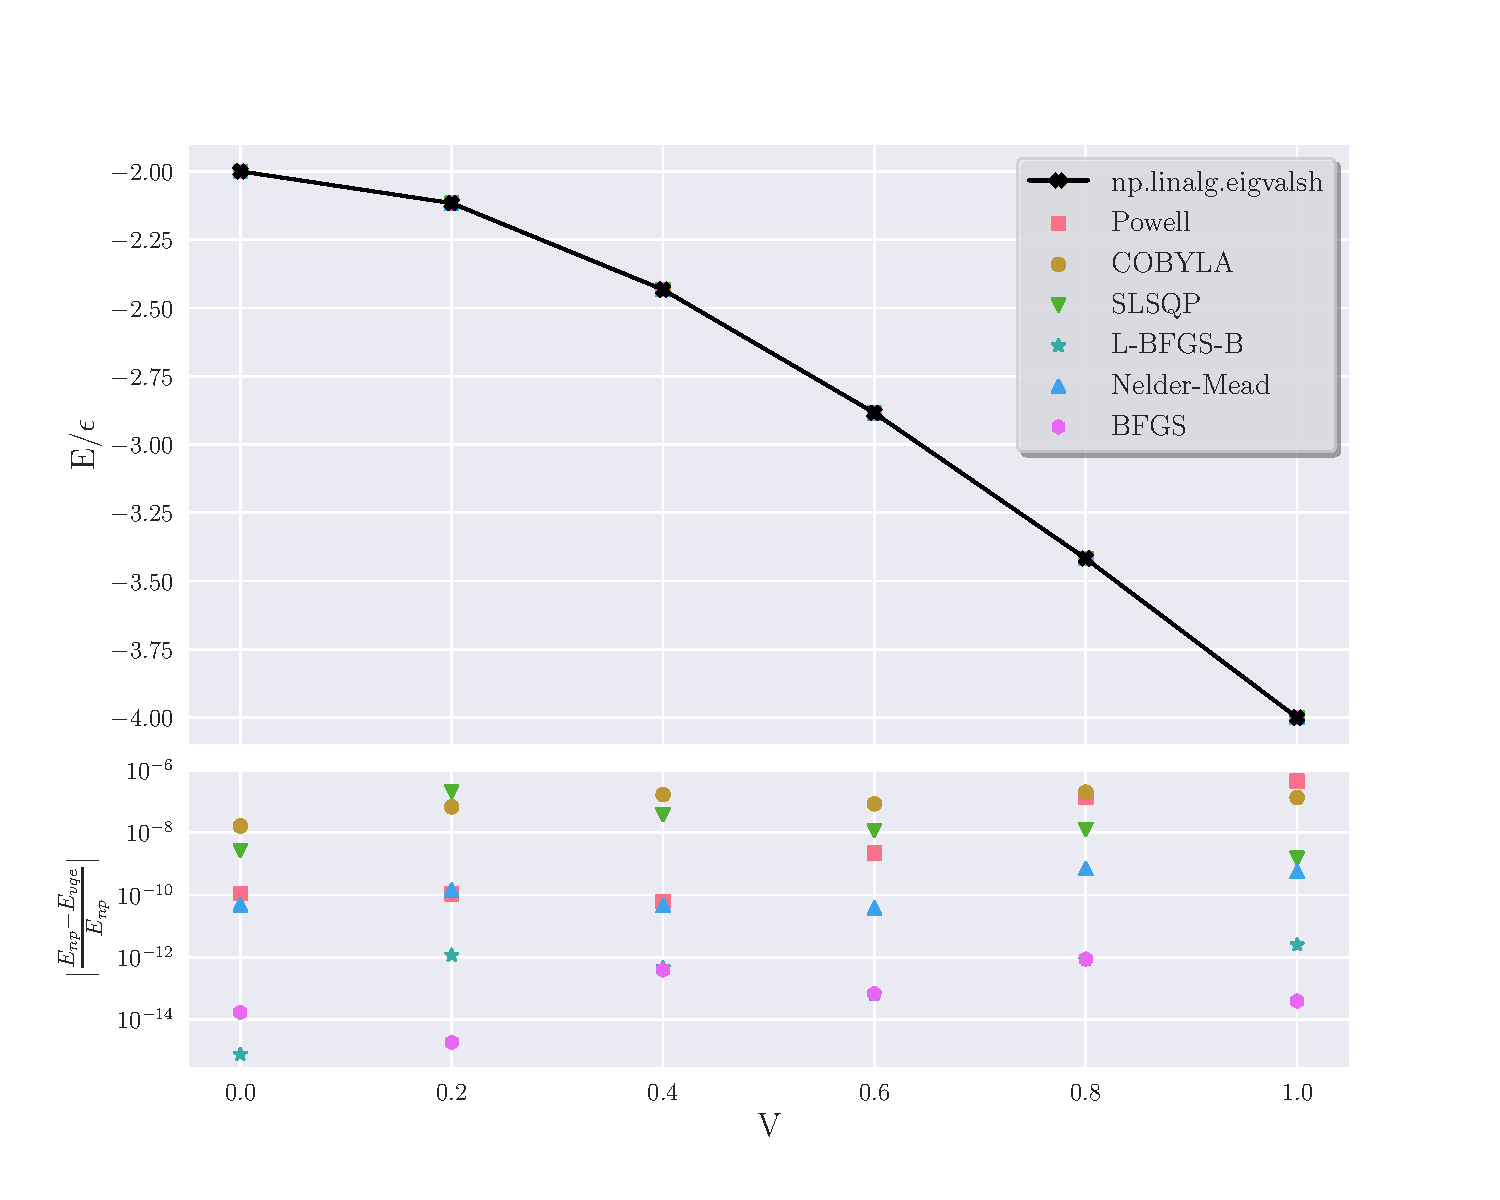
\includegraphics[width=0.47\linewidth]{image/lipkin_result/adapt-opt/cmp_opt_adapt_p_J=2.pdf}
	\caption{Comparison amongst different optimisers for the ADAPT-VQE without shot noise for $ J=1 $ (top) and $ J=2 $ (bottom).}
	\label{fig:OptAdapt}
\end{figure}

\begin{figure}[ht]
	\centering
	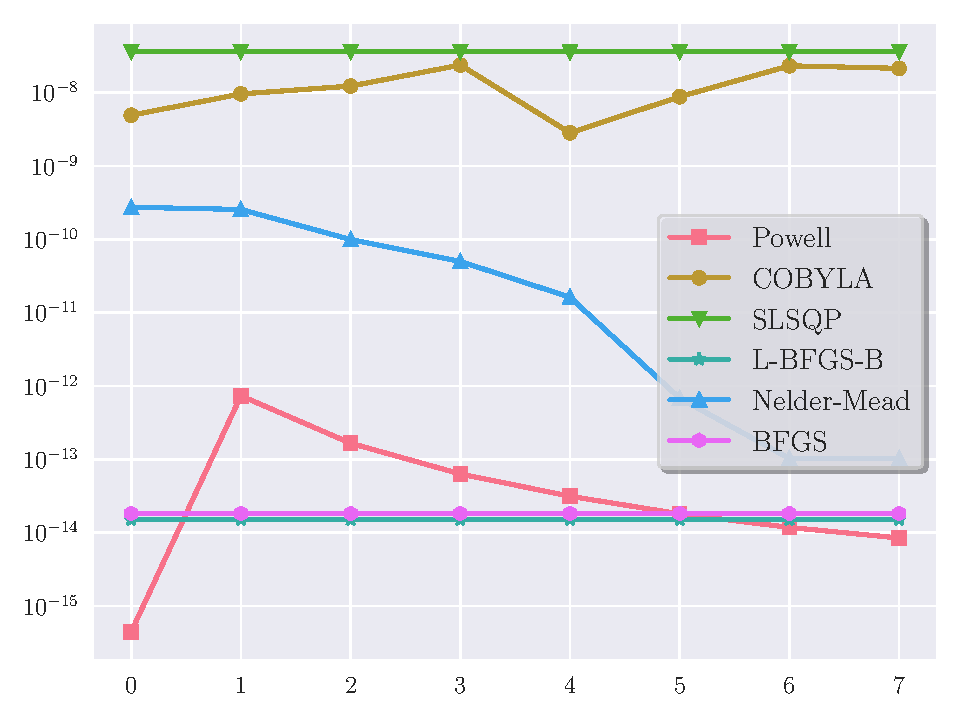
\includegraphics[width=0.47\linewidth]{image/lipkin_result/onlyneed1iter.pdf}
	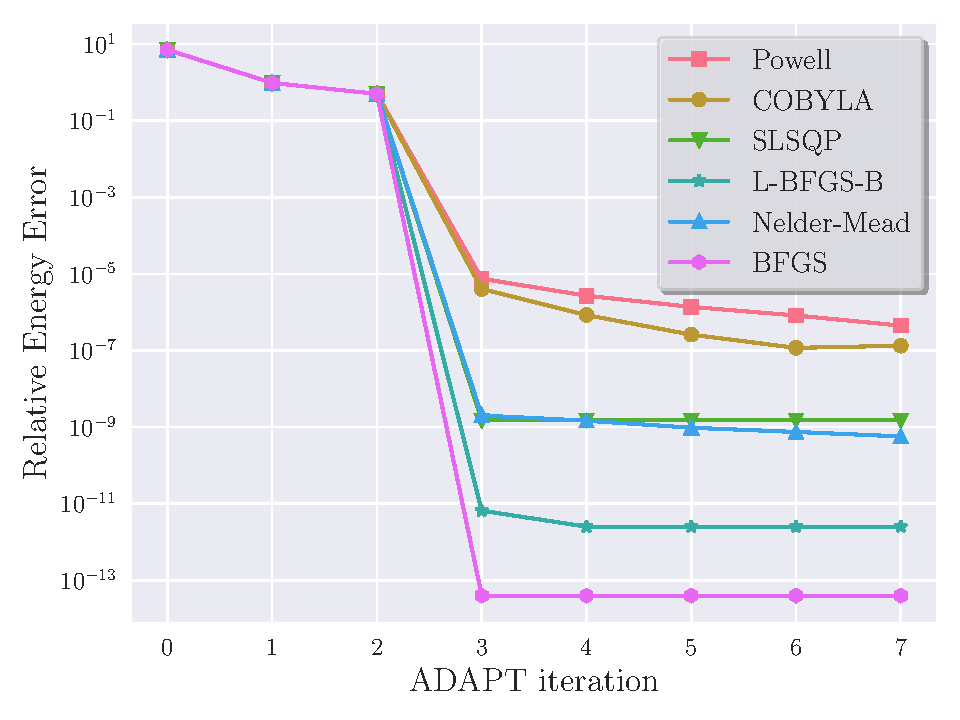
\includegraphics[width=0.47\linewidth]{image/lipkin_result/onlyneed3iter.pdf}
	\caption{Comparison amongst different optimisers for the ADAPT-VQE without shot noise for $ J=1 $ and $ J=2 $.}
	\label{fig:onlyneed1iter}
\end{figure}

As seen in Figure~\ref{fig:onlyneed1iter}, all the optimisers were able to achieve high accuracy with just one iteration for the $ J=1 $ case, and for the $ J=2 $ case it took only $ 3 $ iterations for all ADAPT to converge regardless of the choice of optimisers.

\paragraph{ideal Simulation}

As it turned out, the best optimisers that are robust against shot noise are different from those without shot noise. Whilst we see that all optimisation methods converge to different accuracies for the case without shot noise, some optimisers have shown to be more robust against shot noise. Noticeably, Nelder-Mead takes much longer to converge compared to other methods. 


\begin{table}[ht]
    \centering
    \caption{Optimisersation Results for $ J=1 $ and $ v = 1 $ }
    \label{tab:label}
    \begin{tabular}{c c c c}
	\toprule
	& \textbf{Function Calls} & \textbf{Run Time (s)} & \textbf{Relative Error} \\
	\midrule
	\texttt{COBYLA} & 399 & 2.481 & 0.00268 \\
	\texttt{Powell} & 2475 & 10.849 & 0.01498\\
	\texttt{SQSLP} & 172 & 0.871 & 0.3144 \\
	\texttt{BFGS} & 1160 & 3.749 & 0.286 \\
	\texttt{L-BFGS-B} & 1145 & 4.190 & 0.301  \\
	\texttt{Nelder-Mead} & 219625 & 749.491 & 0.263\\
	\bottomrule
    \end{tabular}
\end{table}

Even for $ N = 10^4 $ shots, most of the optimisers struggle to converge to the correct values. Since only \texttt{COBYLA} and \texttt{Powell} are able to converge to the correct values, they will be the choice of optimisers for the ADAPT-VQE for the main results. Interestingly, they seem to converge to the same values as shown in Figure~\ref{fig:optcmpj1}. 
\begin{figure}[ht]
	\centering
	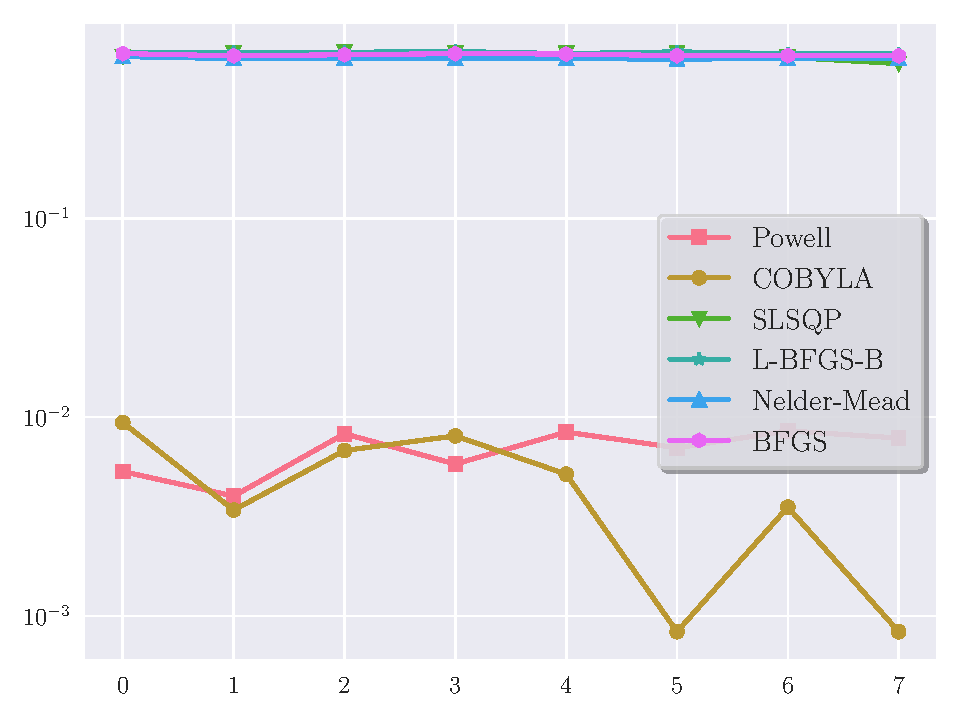
\includegraphics[width=0.45\linewidth]{image/lipkin_result/whynotothersv=0.4.pdf}
	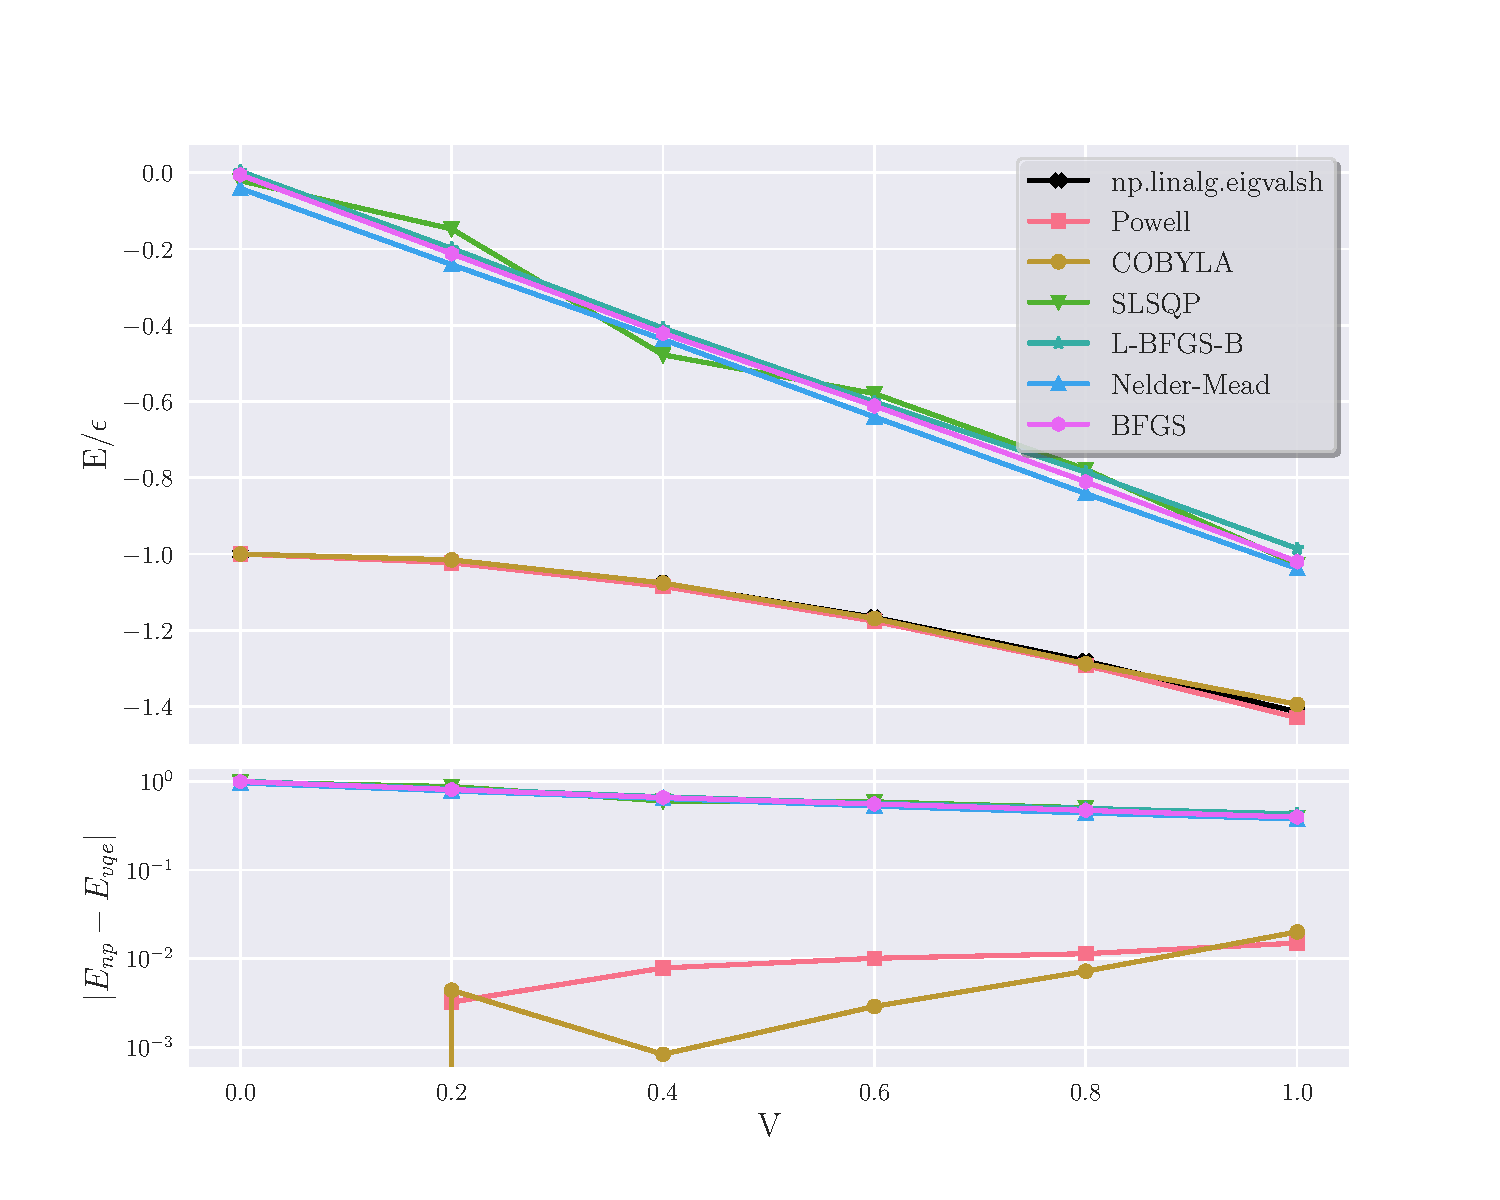
\includegraphics[width=0.45\linewidth]{image/lipkin_result/whynotothers10e4.pdf}	
	\caption{(Left) Comparison amongst different optimisers for the ADAPT-VQE, relative error per ADAPT iterations for $ 8 $ iterations with $ 10e_4 $ shots for $ J=1 $ at $V=0.4$. (Right) Energy plot for different optimisers for different values of $V$.}
	\label{fig:optcmpj1}
\end{figure}

To rule out the possibility that the optimisers which failed to converge were stuck in a local minimum, we could plot the energy landscape for the $ J=1 $ case since there is only one qubit. The energy landscape is shown in Figure~\ref{fig:energy_landscape}. In this case, we only need $ \text{Rx}(\theta) $ and $ \text{Ry}(\phi) $ to span the entire Hilbert space, and the state is then $ R_x(\theta) R_y(\phi)\ket{0}$. The energy landscape shows that there is only a single minimum (within a period), which is the one we are interested in. It is simply a result of the shot noise that the optimisers do not converge properly, which agrees with  Figure~\ref{fig:OptAdapt}, as all the optimisers were able to converge after $ 1 $ iteration.

\begin{figure}[ht]
	\centering
	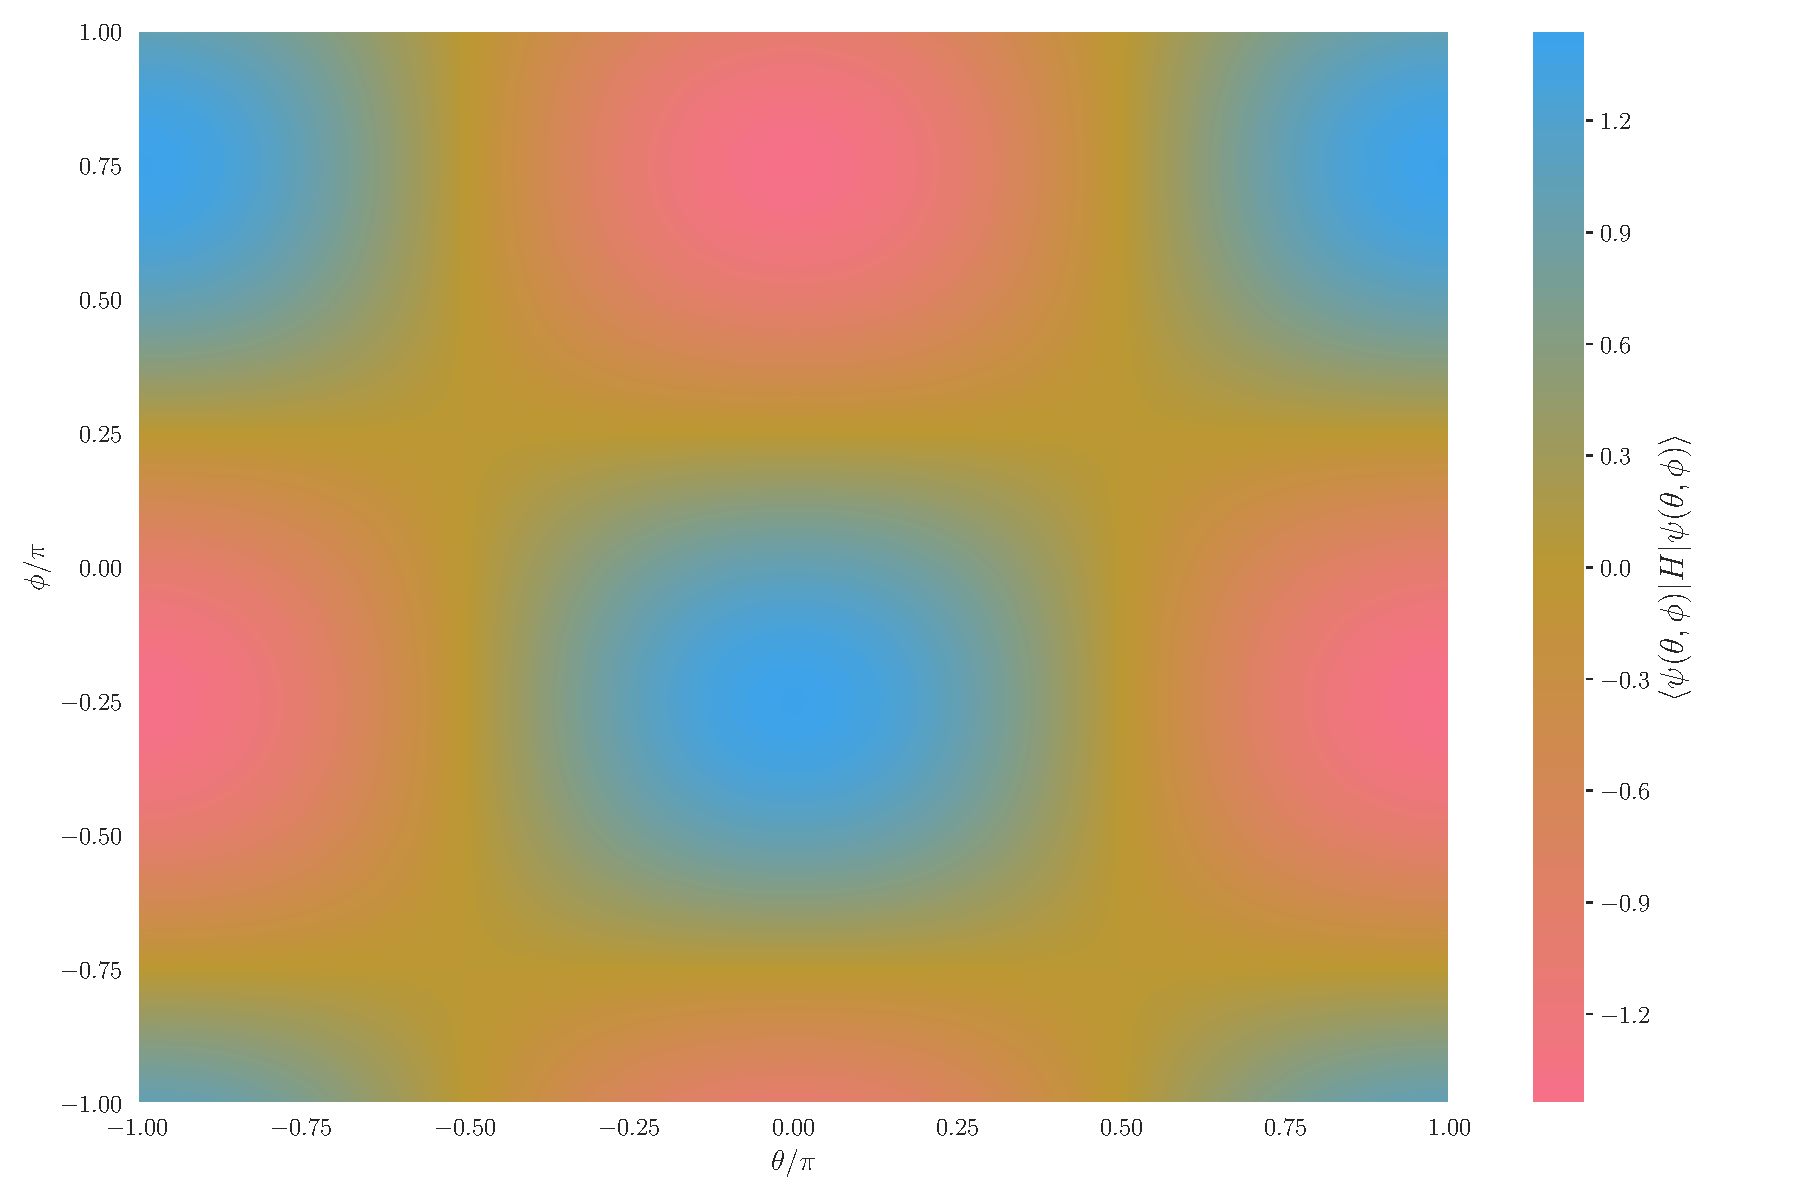
\includegraphics[width=\linewidth]{image/lipkin_result/energy_landscape.pdf}
	\caption{Energy landscape for $J=1$ with $V=1$. } 
	\label{fig:energy_landscape}
\end{figure}



\section{Pairing Model}
\label{sec:pairing_result}
In this section, we show the results of the Pairing model with 4 doubly degenerate states and $ 4 $ particles for both the exact energy and ideal simulation. There are $ 18 $ terms in the qubit Hamiltonian for the pairing model. Therefore the expected error for the pairing model is $ 0.013 $. We have chosen $ \xi = 1 $ and the energy plotted is normalised by $ \xi $ and is hence unitless.

\begin{figure}[ht]
    \centering
    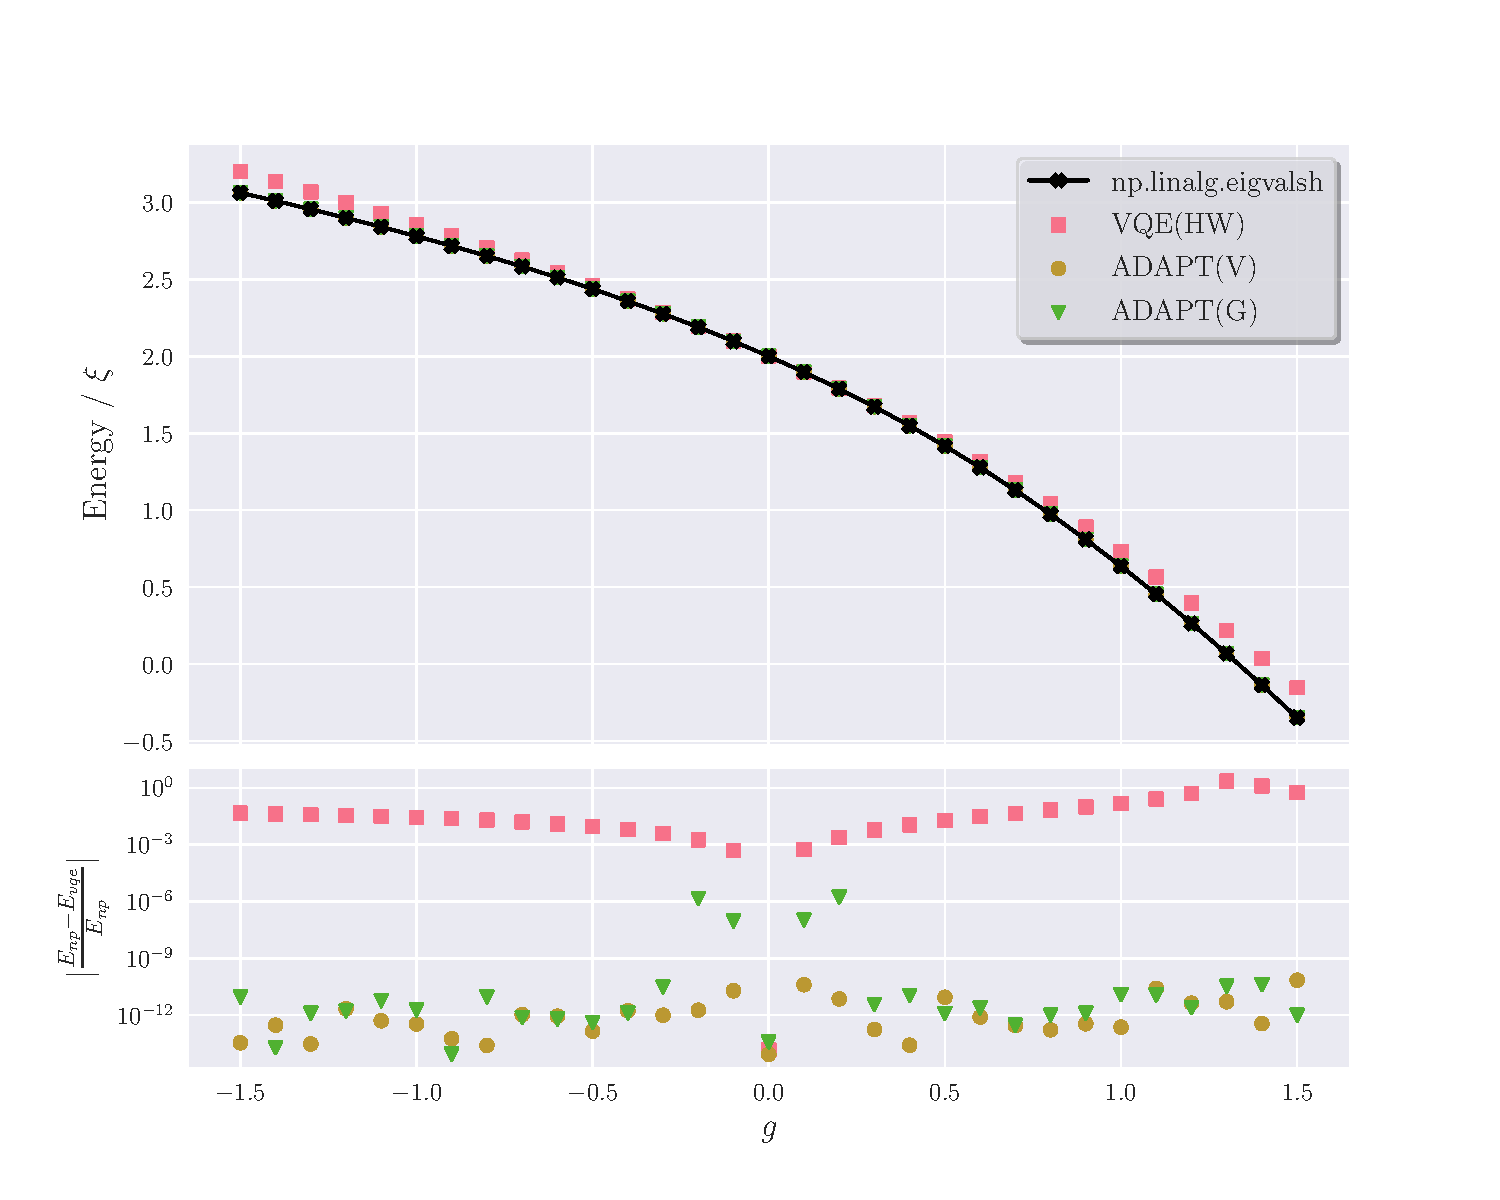
\includegraphics[width=\linewidth]{image/pairing_result/no_shot_noise/pairing-main-result.pdf}
    \caption{\textbf{Exact energy simulation} for the pairing model with \texttt{BFGS} optimiser for both the ADAPT-VQE and the VQE for a maximum of $ 8 $ iterations and $ g \in[-1.5,1.5] $. The hardware efficient ansatz with 2 repetitions was used for the VQE.}
    \label{fig:small-main}
\end{figure}

We first look at the results for $ g \in [-1.5, 1.5] $ for the ADAPT-VQE with both the $ V $ pool and the $ G $ pool, as well as the hardware efficient ansatz. As we can see from Figure~\ref{fig:small-main}, when exact energy is calculated, the ADAPT-VQEs with both pools were able to converge to the exact energy diagonalisation n with errors of orders of $ 10^{-9} $ for $ g \in [-1.5, 1,5] $ for only $ 8 $ maximum iterations. The $G$ pool performd slightly worse (with error $ \sim \mathcal{O}(10^{-6}) $ ) for values close to $ 0 $. The hardware efficient ansatz was not able to obtain the same level of accuracies as the ADAPT-VQE, but the relative error was consistent for most of the values of $ g $ in orders of $ 10^{-2} $, with the exception of $ g = 0$ where the Hamiltonian given by Equation~\eqref{eq:pairing-mat} is diagonal, which the hardware efficient ansatz was able to represent exactly.

\begin{figure}[ht]
    \centering
    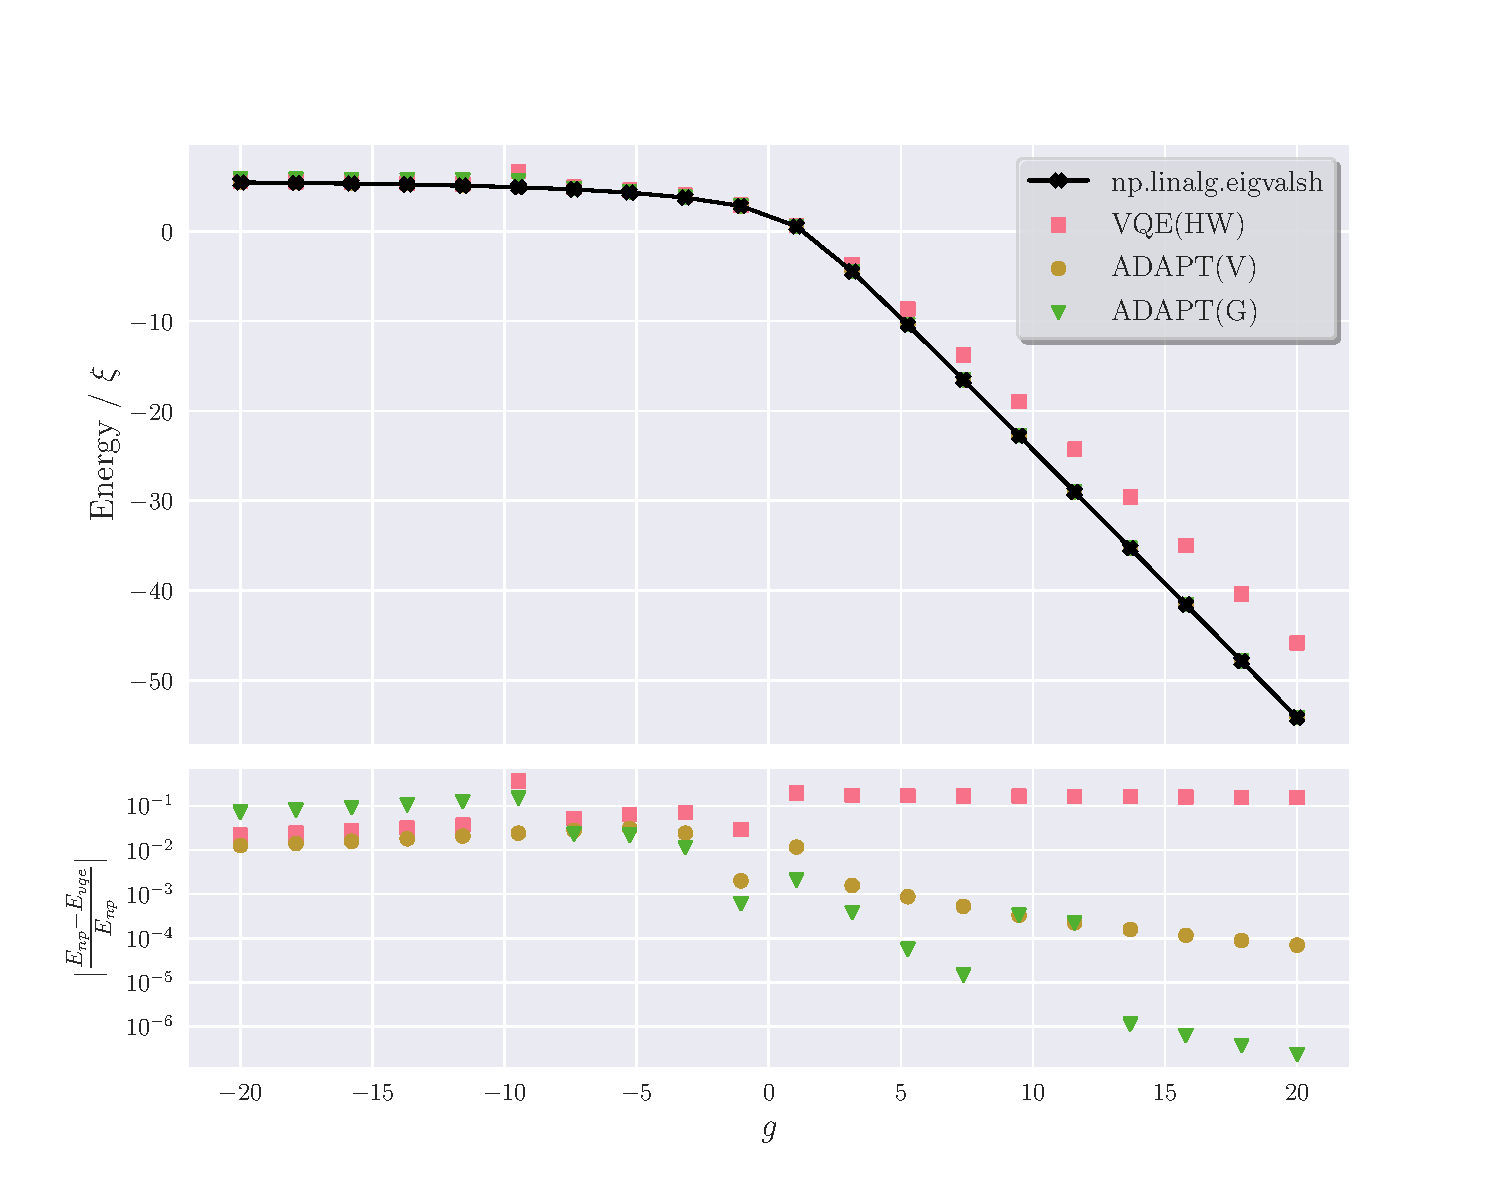
\includegraphics[width=\linewidth]{image/pairing_result/no_shot_noise/sameparams-big.pdf}
    \caption{\textbf{Exact energy simulation} for the pairing model with \texttt{BFGS} optimiser for both the ADAPT and the normal VQE for a maximum of $ 6 $ iterations and $ g \in[-20,20] $. The HW ansatz with 2 repetitions was used for the VQE.}
    \label{fig:big-main}
\end{figure}


We ran the exact energy simulation again for $ g \in [-20,20] $, as shown in Figure~\ref{fig:big-main}. The number of maximum iterations was set to $ 6 $ to match the parameter in the hardware efficient ansatz with $ 2 $ repetitions. For values of $ g \in [-20,0] $, the ADAPT-VQEs performed similarly to the VQE, with an error between $ 10^{-2} $ to $ 10^{-1} $. However, for large pairing strength $ g $, the ADAPT-VQEs perform much much better than the VQE. The reason why the ADAPT-VQEs do not perform as well for the negative region of $ g $ could be due to the fact that $ 6 $ maximum iterations were not enough for the ADAPT-VQE to converge. Another point worth noting is that the bottom plot in Figure~\ref{fig:big-main} is the relative error. As the energy increases, the energy increases in magnitude, and the relative error takes account into the fact of the changing magnitude of the energy, making it a better indicator than the absolute error for algorithmic performance. 

\begin{figure}[ht]
    \centering
    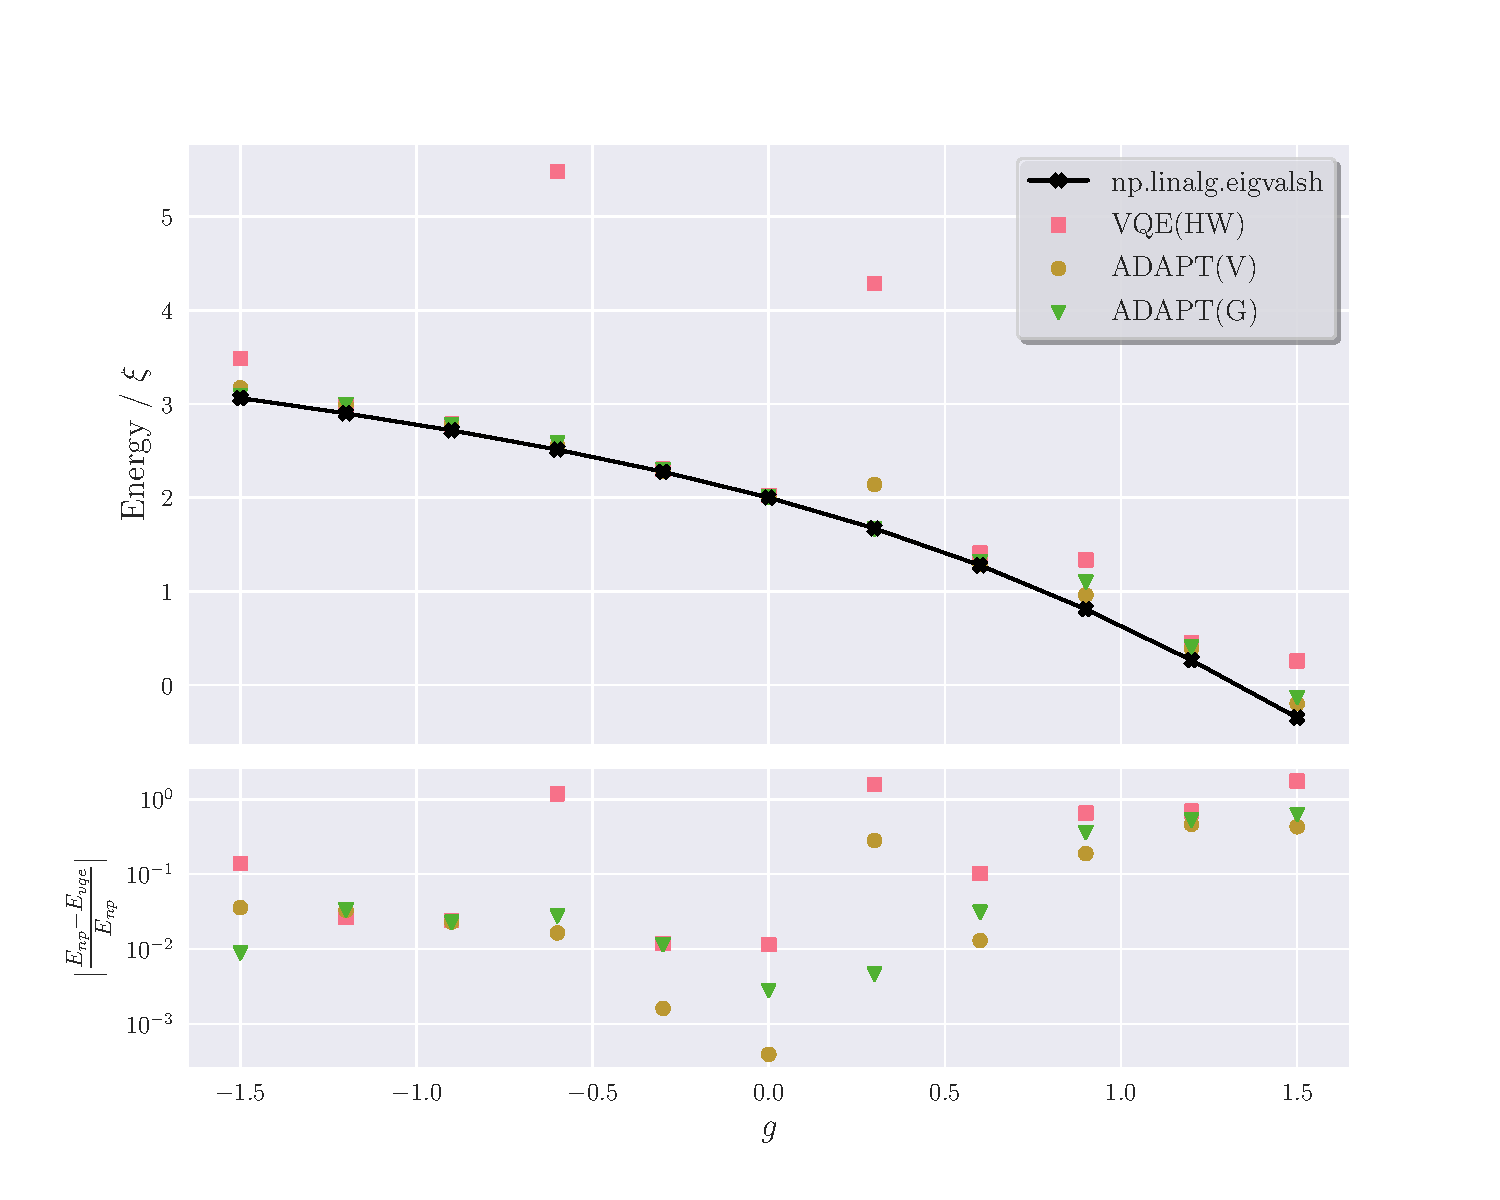
\includegraphics[width=\linewidth]{image/pairing_result/ideal simulation/noisy-16-sm.pdf}
    \caption{\textbf{Ideal Simulation} for the pairing model with \texttt{COBYLA} method for the ADAPT-VQEs and \texttt{Powell} for the VQE for a maximum of $ 16 $ iterations for $ g \in[-1.5,1.5] $. The hardware efficient ansatz with 2 repetitions is used for the VQE.}
	\label{fig:small-main-noisy}
\end{figure}
\begin{figure}[ht]
    \centering
    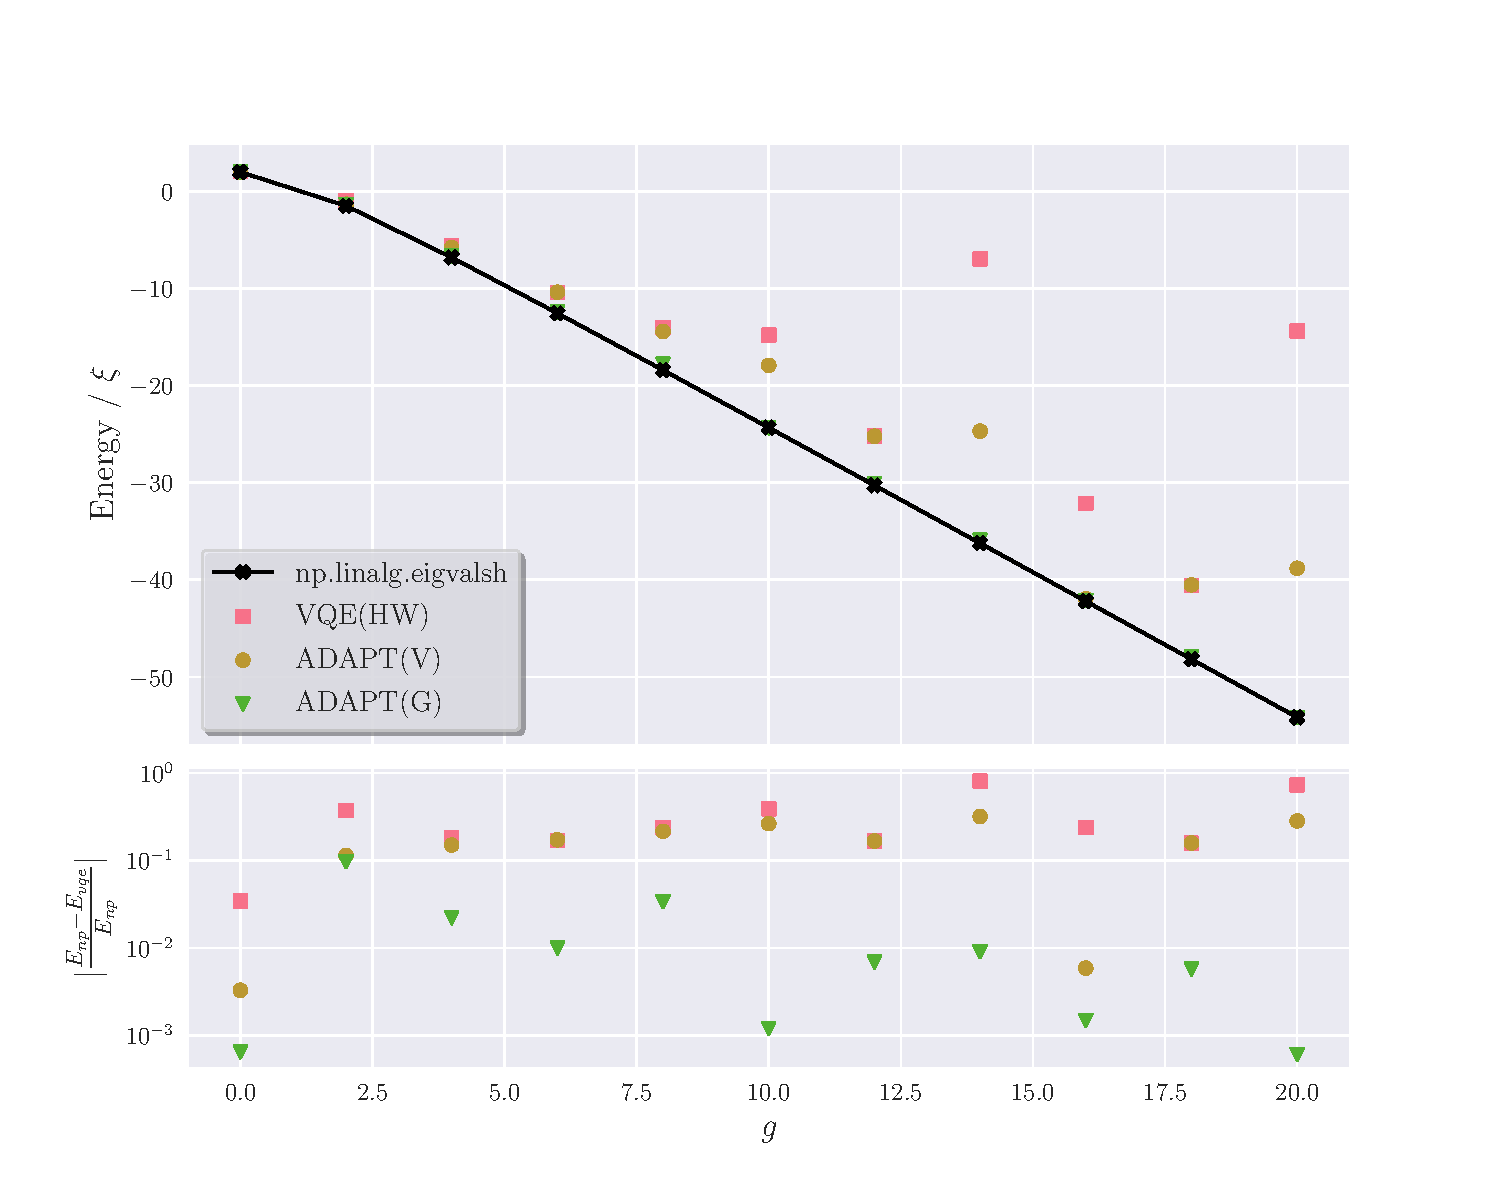
\includegraphics[width=\linewidth]{image/pairing_result/ideal simulation/noisy-16-big.pdf}
    \caption{\textbf{Ideal Simulation} for the pairing model with \texttt{COBYLA} method for the ADAPT-VQE and \texttt{Powell} for the VQE for a maximum of $ 16 $ iterations for $ g \in[0,20] $} 
    \label{fig:big-main-noisy}
\end{figure}

Figure~\ref{fig:small-main-noisy} shows the results for the ideal simulation of the pairing model. We expected that by including shot noise the ADAPT-VQEs would require more iterations to converge, hence the maximum iteration was increased to $ 16 $.

For $ g \in [-1.5, 1.5]$, the results produced with both ADAPT-VQEs and the VQE performed similarly in terms of accuracies. However, the ADAPT-VQEs were more consistent in convergence to the ground state while for many points the VQE did not manage to converge. This is aligned with the analysis we performed earlier for the LMG model for Figures~\ref{fig:j2main-nsn} and~\ref{fig:j2main-noisy} where for some points the VQE with hardware efficient ansatz failed to converge. 

Results for ideal simulation for $ g \in [0,20] $ are presented in Figure~\ref{fig:big-main-noisy}. This is the only time we observed a difference in the performance of the pools. We observed similar results in Figure~\ref{fig:big-main} but fewer iterations were allowed and the differences were not as clear. The $ G $  pool consistently outperformed the $ V $  pool in the interval $ g \in [0,20] $, with errors within orders of $ 10^{-2} $, while the V pool performed similarly to the VQE with hardware efficient ansatz. Looking into the details we included $ 2 $ ADAPT iteration graphs shown in Figure~\ref{fig:8-16-iter} for $ g=8 $ and $ g=16 $ respectively. In both cases, the $ G $ pool found the operators which allowed it to converge after just a couple of iterations, whereas for the $ V $ pool, appending new operators did not improve the energy. For the $ g=8 $ case, the $ V $ pool did not converge at all and for the $ g=16 $ case, the energy started to decrease at around $ 11 $ iterations, much later than the $ G $ pool. Looking at the structure of the pools as presented in equations~\eqref{eq:gpool} and ~\eqref{eq:vpool}, we could see that the operators in the $ G $ pool have a localised structure but it is unclear what was the cause of the difference in performance.

\begin{figure}[ht]
    \centering
    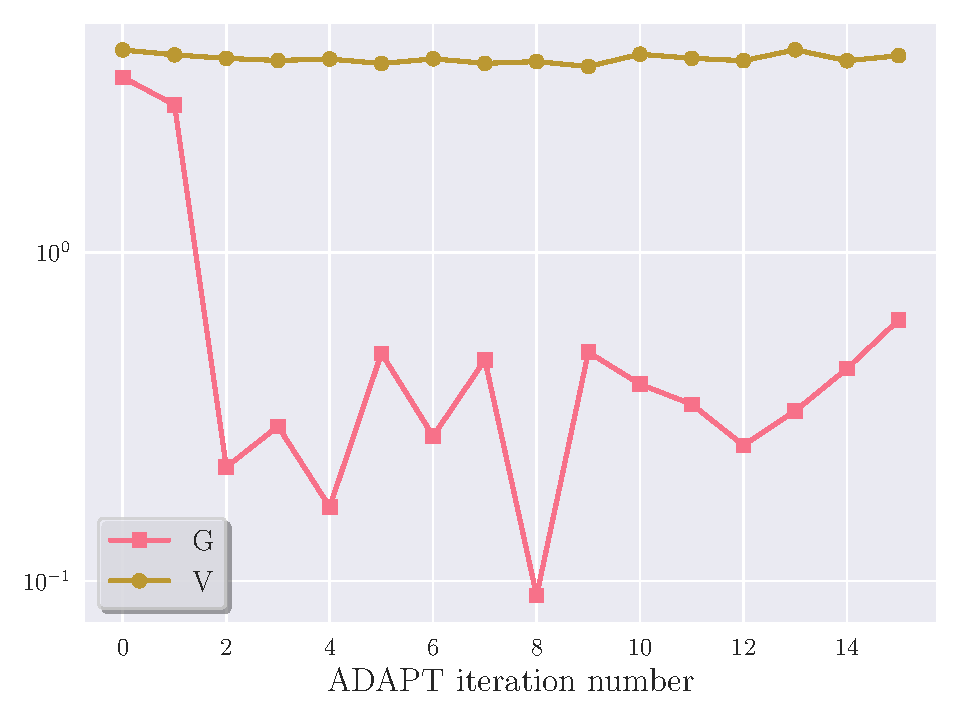
\includegraphics[width=0.45\linewidth]{image/pairing_result/ideal simulation/g8.pdf}
    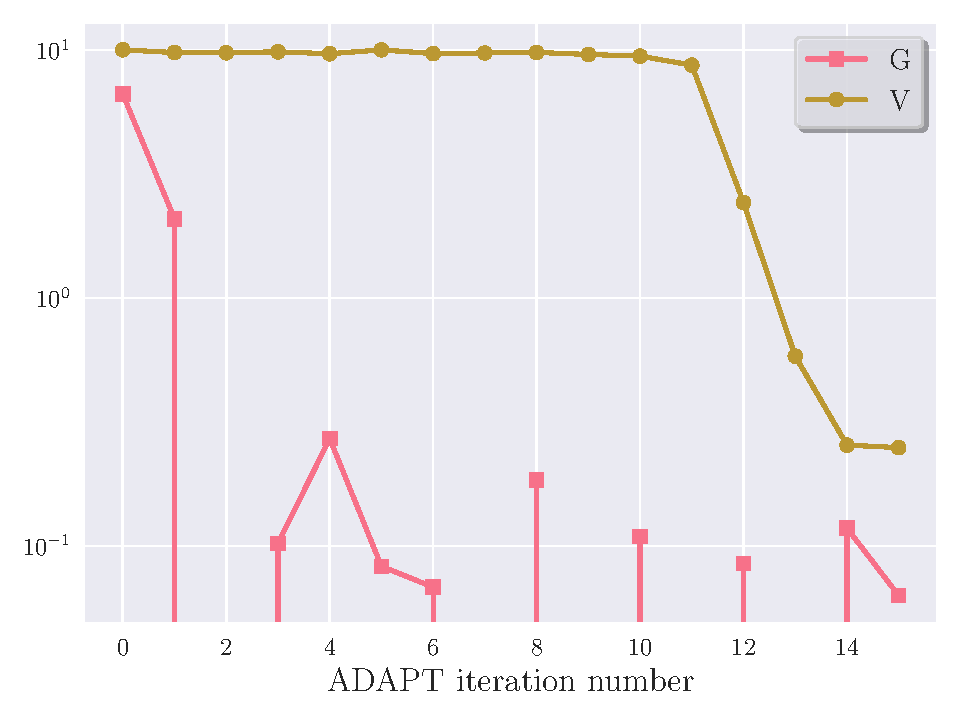
\includegraphics[width=0.45\linewidth]{image/pairing_result/ideal simulation/g=16adaptiter.pdf}
    \caption{ADAPT-VQE error at every iteration for the pairing model using \texttt{COBYLA} optimiser for $ g=16 $ (left) and $ g=18 $ (right).}
    \label{fig:8-16-iter}
\end{figure}


\section{Deuteron Model}
\label{sec:deuteron_result}


In this section, we present both the exact energy simulation and ideal simulation results for the deuteron model for different numbers of basis dimensions $ N $. We compare our results to the numerical diagonalisation using $ numpy.linalg.eigvalsh$. For the deuteron model with $ N=n $, the number of qubits required is $ \lceil \log_2( n ) \rceil$. Unlike the other models we have simulated, the qubit Hamiltonians of the deuteron model will have a different number of terms for different values of $ N $, and the expected error depends on $ N $ as well. This is an interesting case to include as we can easily compare the performance for different numbers of qubits for the same system. 
The numbers of terms in the Hamiltonian are $ 8,20$ and $48 $ for the $ 2,3$ and $4$ qubit cases respectively, so the expected error for these cases should be $ \mathcal{O}(10^{-2}) $.

\subsection{Exact Energy Simulation}
We first look at the results for $ N \in [2,32] $ for the exact energy simulation. 

\begin{figure}[ht]
    \centering
    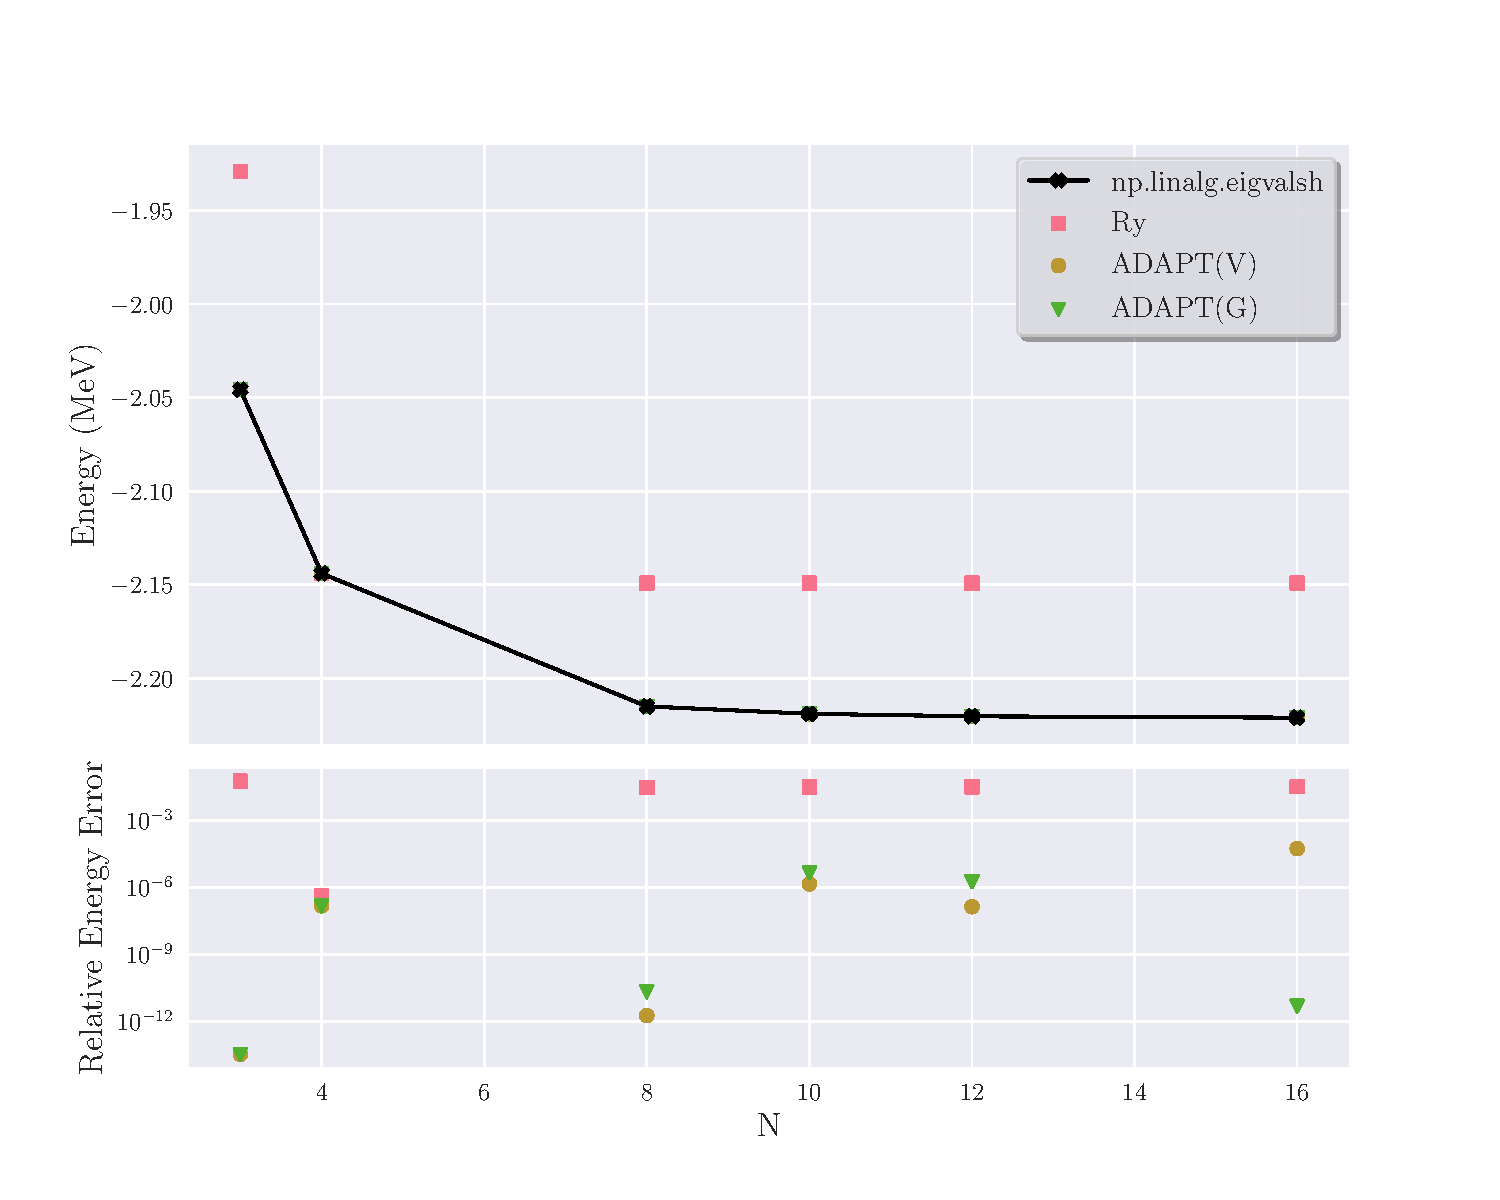
\includegraphics[width=\linewidth]{image/deuteron_result/main1.pdf}
    \caption{The deuteron model with \textbf{exact energy simulation} for $ N \in [3,16] $ with the \texttt{BFGS} optimiser for the ADAPT-VQE for a maximum of $ 16 $ iterations.}
    \label{fig:deuteronmain}
\end{figure}
Again, we saw that the errors obtained using the VQE with hardware efficient ansatz stay around $ 10^{-2} $, even for more qubits. While the ADAPT-VQEs were outperforming the VQE by a large margin for cases with few qubits, as the number of qubits grew, this margin reduced drastically. For $ N=32 $, the ADAPT-VQEs both have errors in orders of $ 10^{-4} $. This is likely due to the fact that as the number of qubits grows, the number of operators needed to represent the ground state also grows. Since the minimum size of a complete pool grows linearly with the number of qubits, the number of operators in the ansatz to represent the ground state should grow linearly as well. We will investigate this further in the Subsection~\ref{sub:itervsqubits}. 

\subsection{Ideal Simulation}
\begin{figure}[ht]
	\centering
	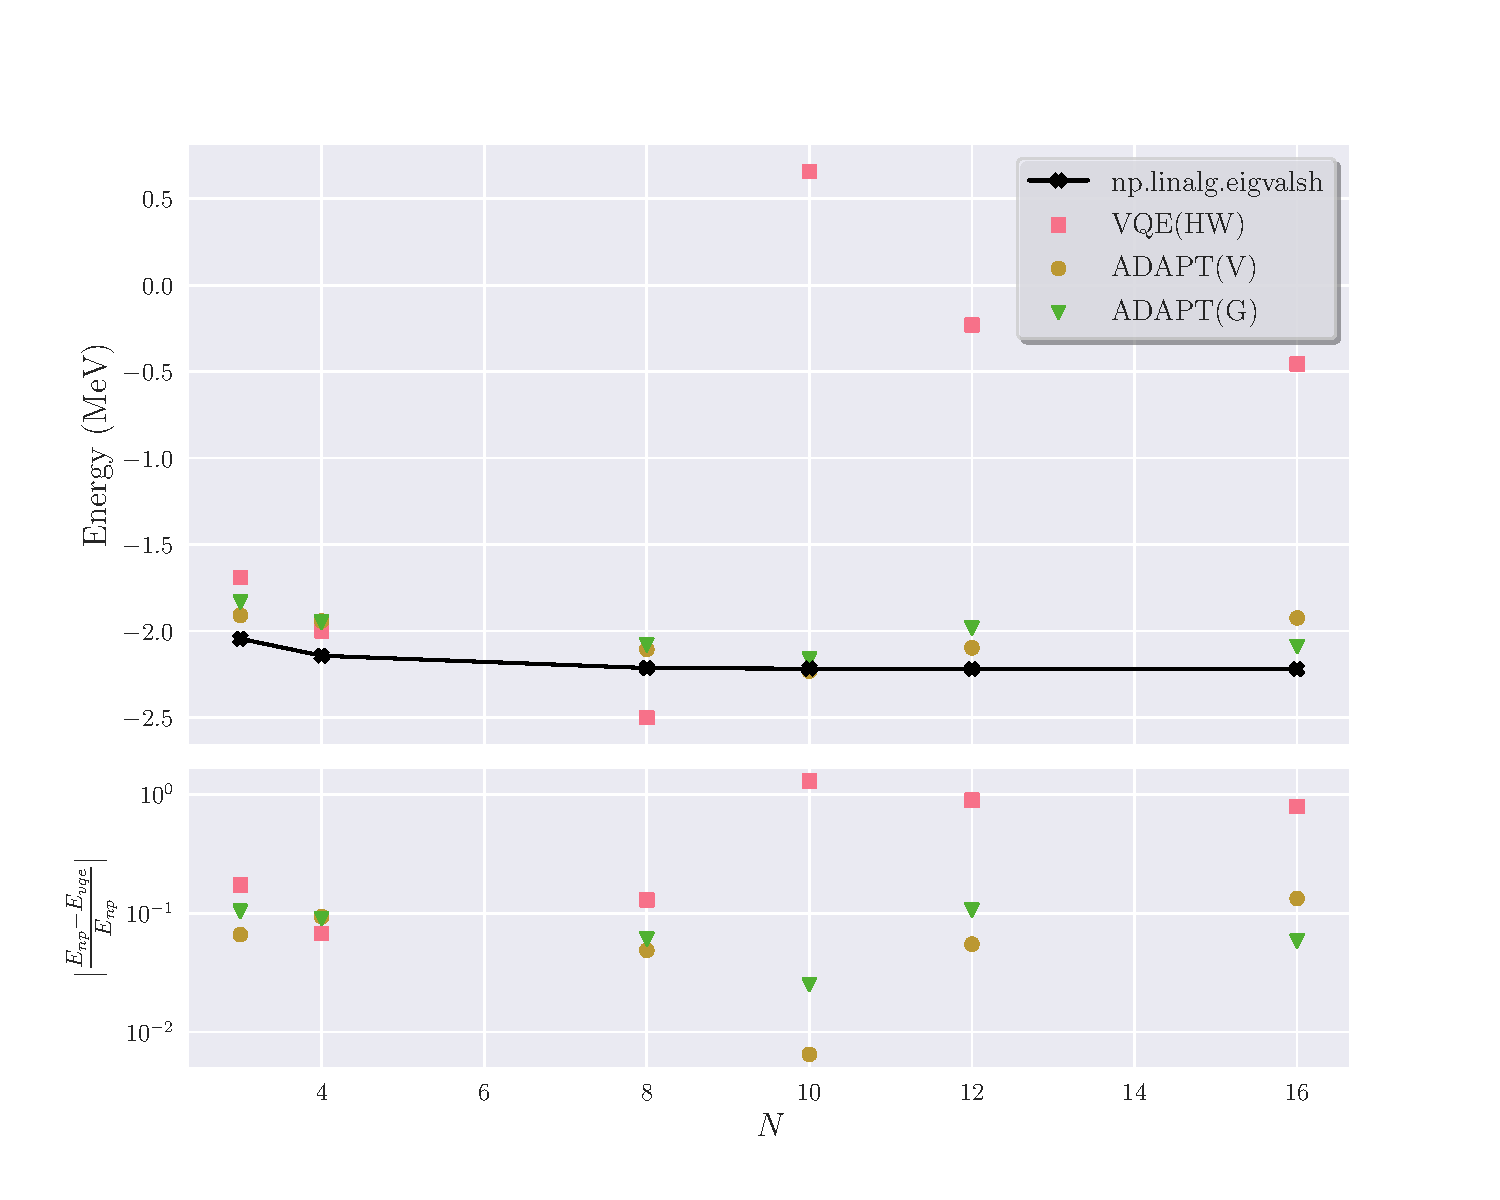
\includegraphics[width=\linewidth]{image/deuteron_result/main2.pdf}
	\caption{The deuteron model with \textbf{ideal simulation} for $ N \in [3, 16] $ with the \texttt{COBYLA} optimiser for the ADAPT-VQE for a maximum of $ 16 $ iterations.}
	\label{fig:deuteronmain-noisy}
\end{figure}

\subsection{Scaling of Iterations with Number of Qubits}
\label{sub:itervsqubits}

How many ADAPT iterations in the exact energy simulation do we expect the qubit-ADAPT-VQE to need to converge? We ran the exact energy simulation for the deuteron model for $ 1 $ to $ 7 $ qubits, using the \texttt{SLSQP} optimiser. The results are shown in Figure~\ref{fig:howmany}. Combining this with Figure~\ref{fig:onlyneed1iter} we could see the number of iterations required for the ADAPT-VQE to converge is independent of the optimisers used but rather the number of the qubits in the system as shown in Figure~\ref{fig:howmany}. We summarised the results in Table~\ref{tab:howmany}. Interestingly, the number of iterations grows much faster for a lower number of qubits, and as the number of qubits increases, the number of iterations required to converge increases at a much slower rate, seemingly linearly. Due to the large amount of time required to run this simulation, we will not be able to run the convergence test for more qubits. However, if the number of iterations required for the convergence does not grow as fast as the number of qubits, then both the QubitAdaptAnsatz and the ADAPT-VQE will scale nicely into larger systems.


\begin{table}[ht]
    \centering
    \caption{Number of iterations required for the ADAPT-VQE to converge for different numbers of qubits.}
    \label{tab:howmany}

    \begin{tabular}{c c c}
	\toprule
	\textbf{N} & \textbf{Number of Qubits} & \textbf{Number of Iterations} \\
	\midrule
	2 & 1 & 1 \\
	4 & 2 & 2 \\
	8 & 3 & 6 \\
	16 & 4 & 8 \\
	32 & 5 & 9 \\
	64 & 6 & 11 \\
	128 & 7 & 12 \\
	\bottomrule
    \end{tabular}
\end{table}
\begin{figure}[ht]
    \centering
    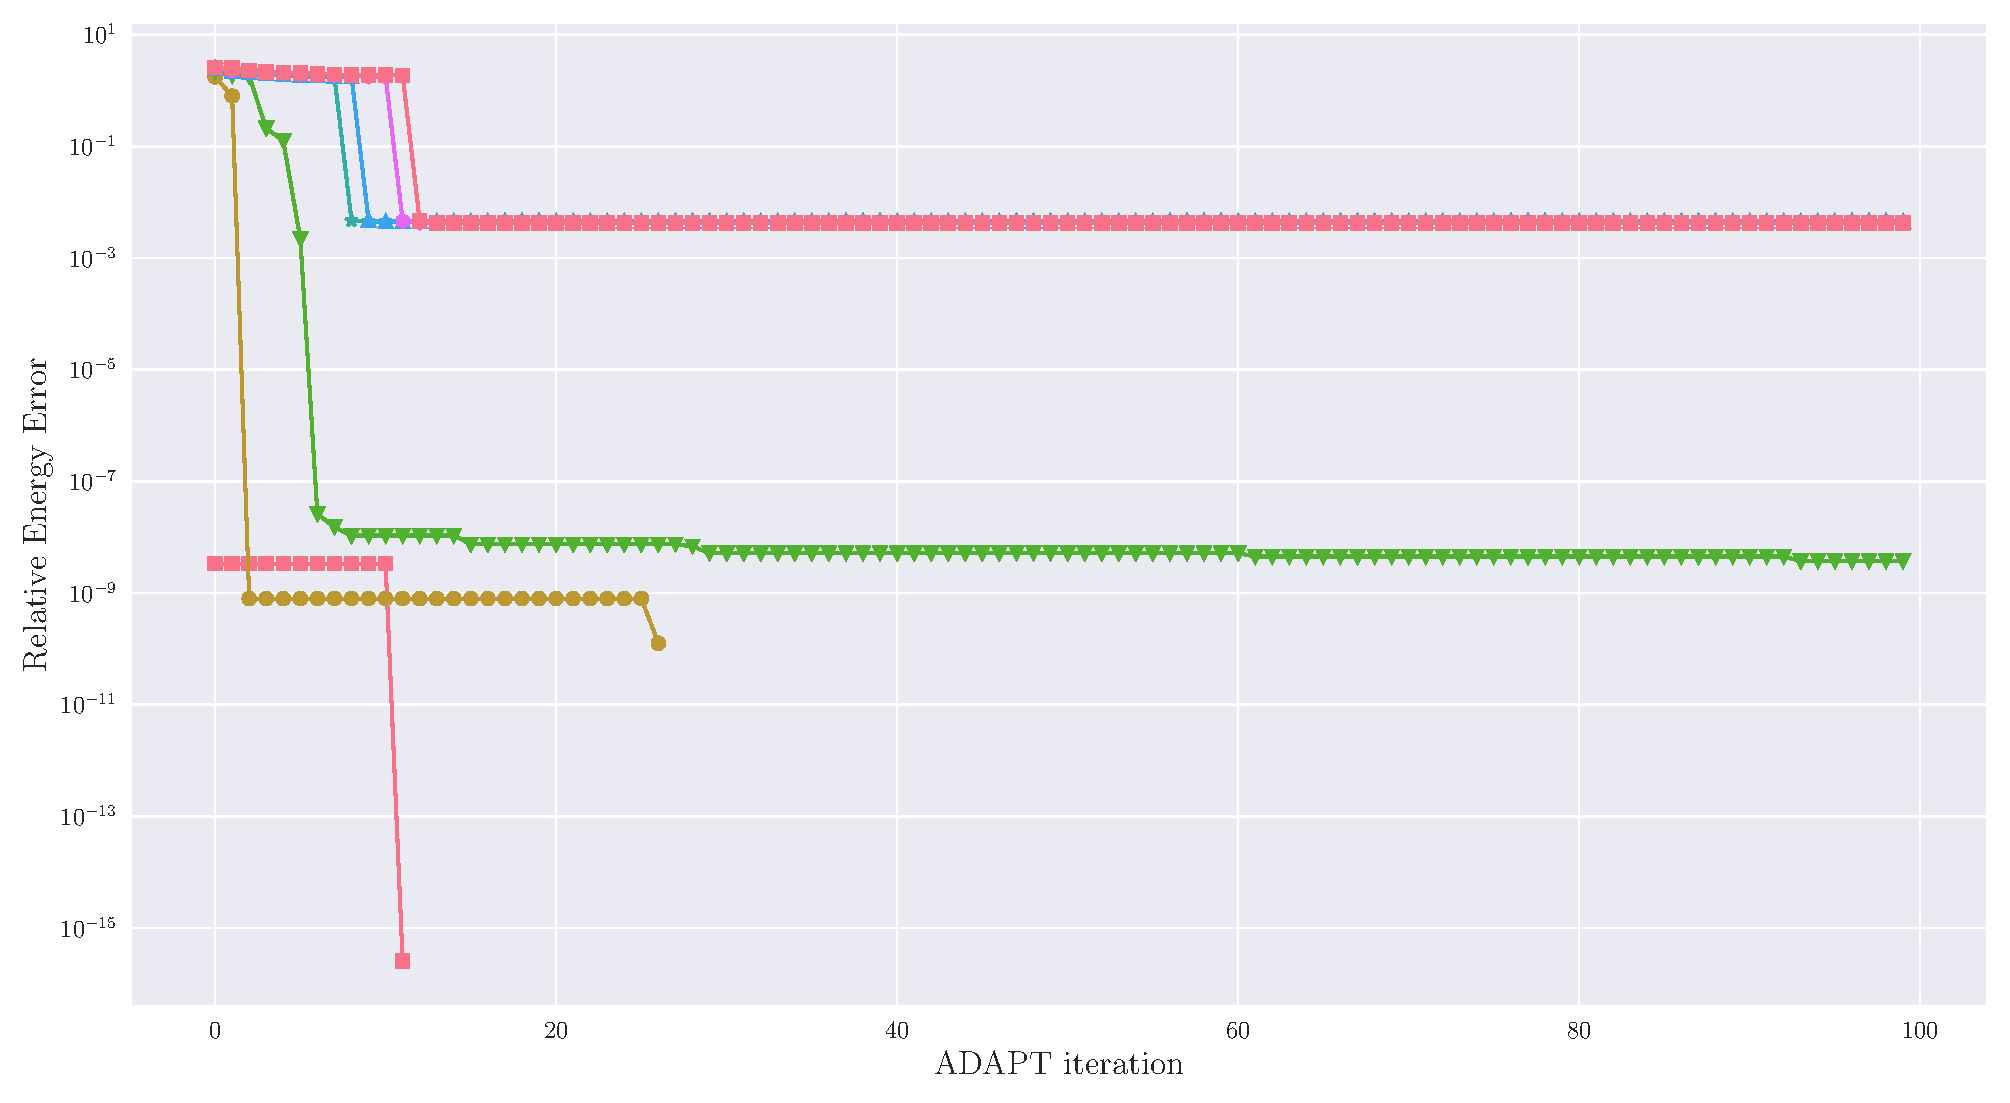
\includegraphics[width=0.8\linewidth]{image/deuteron_result/howmanyiters_whole.pdf}
    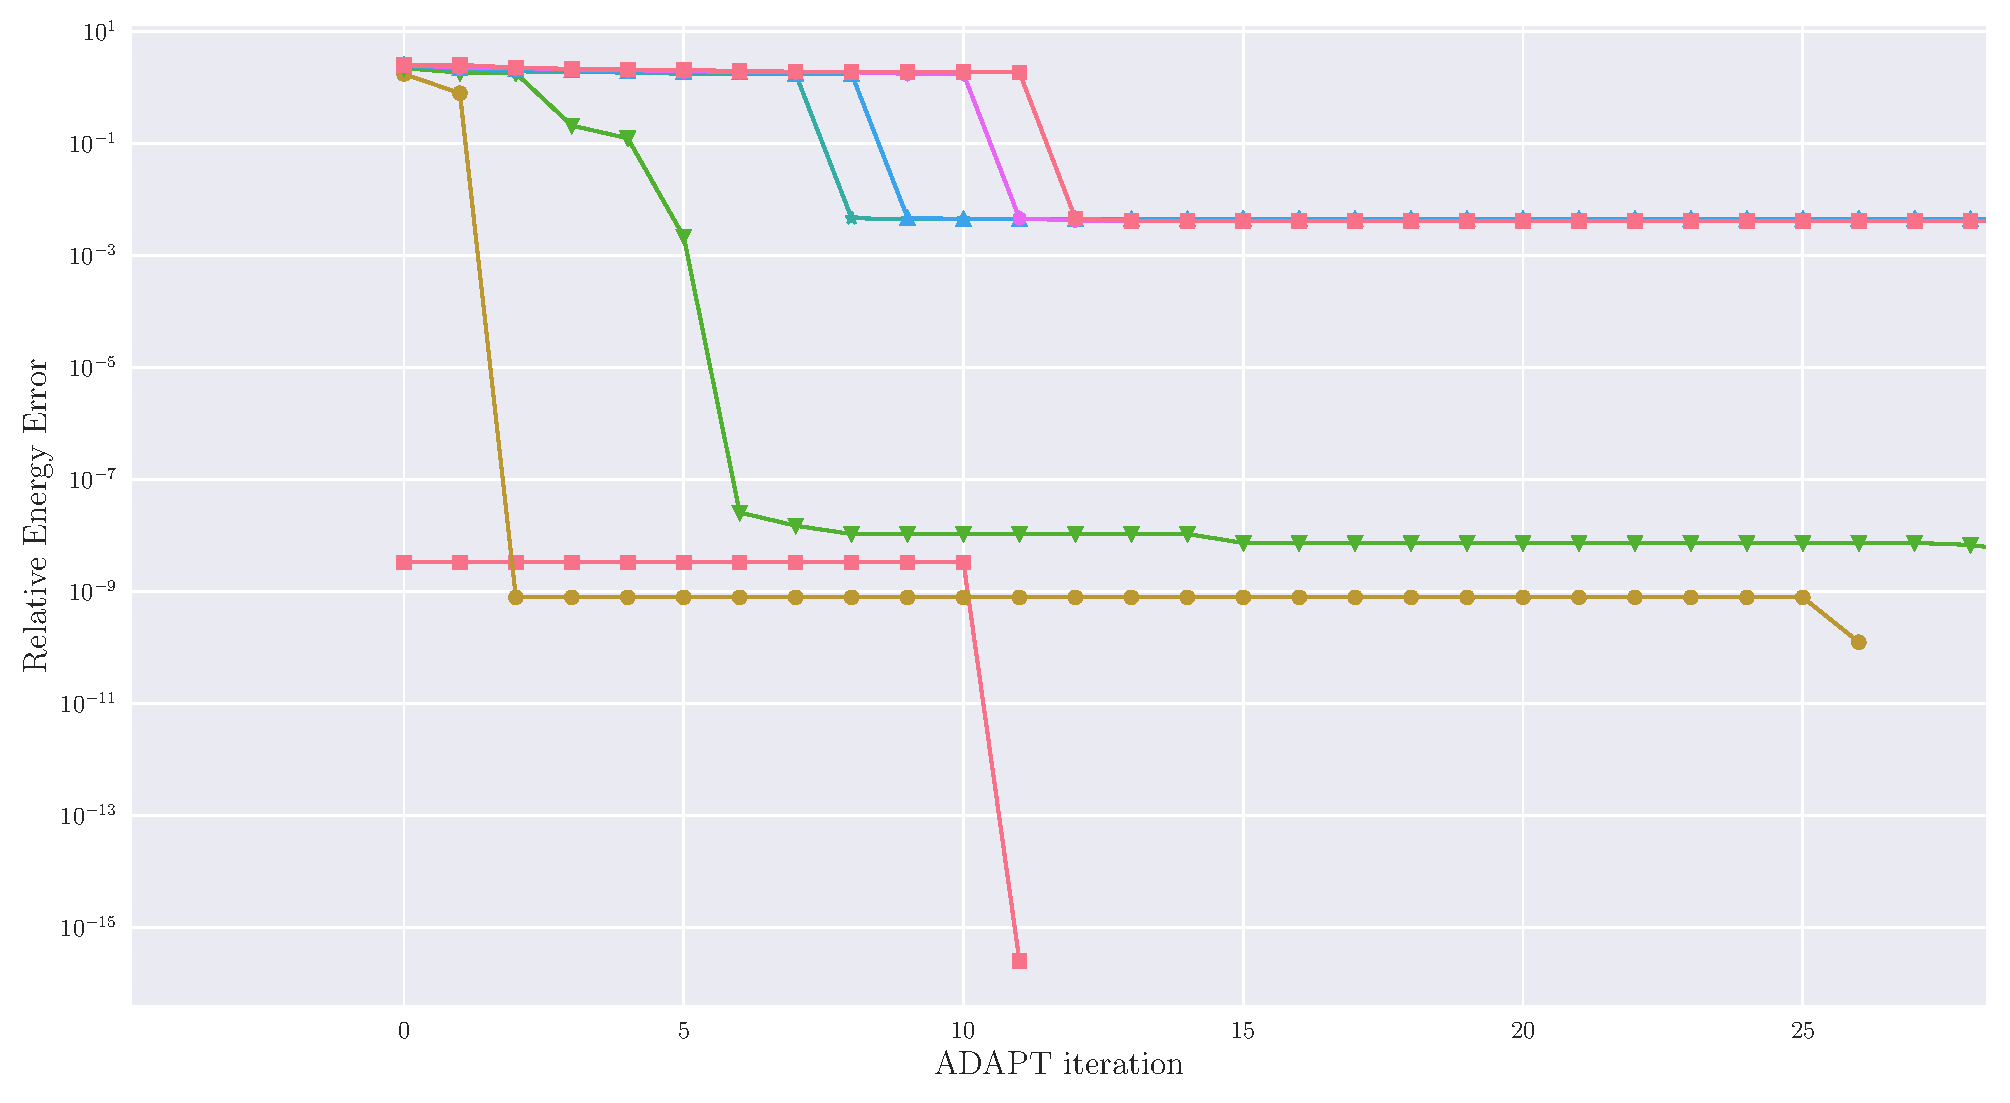
\includegraphics[width=0.8\linewidth]{image/deuteron_result/howmanyiters_zoom.pdf}
    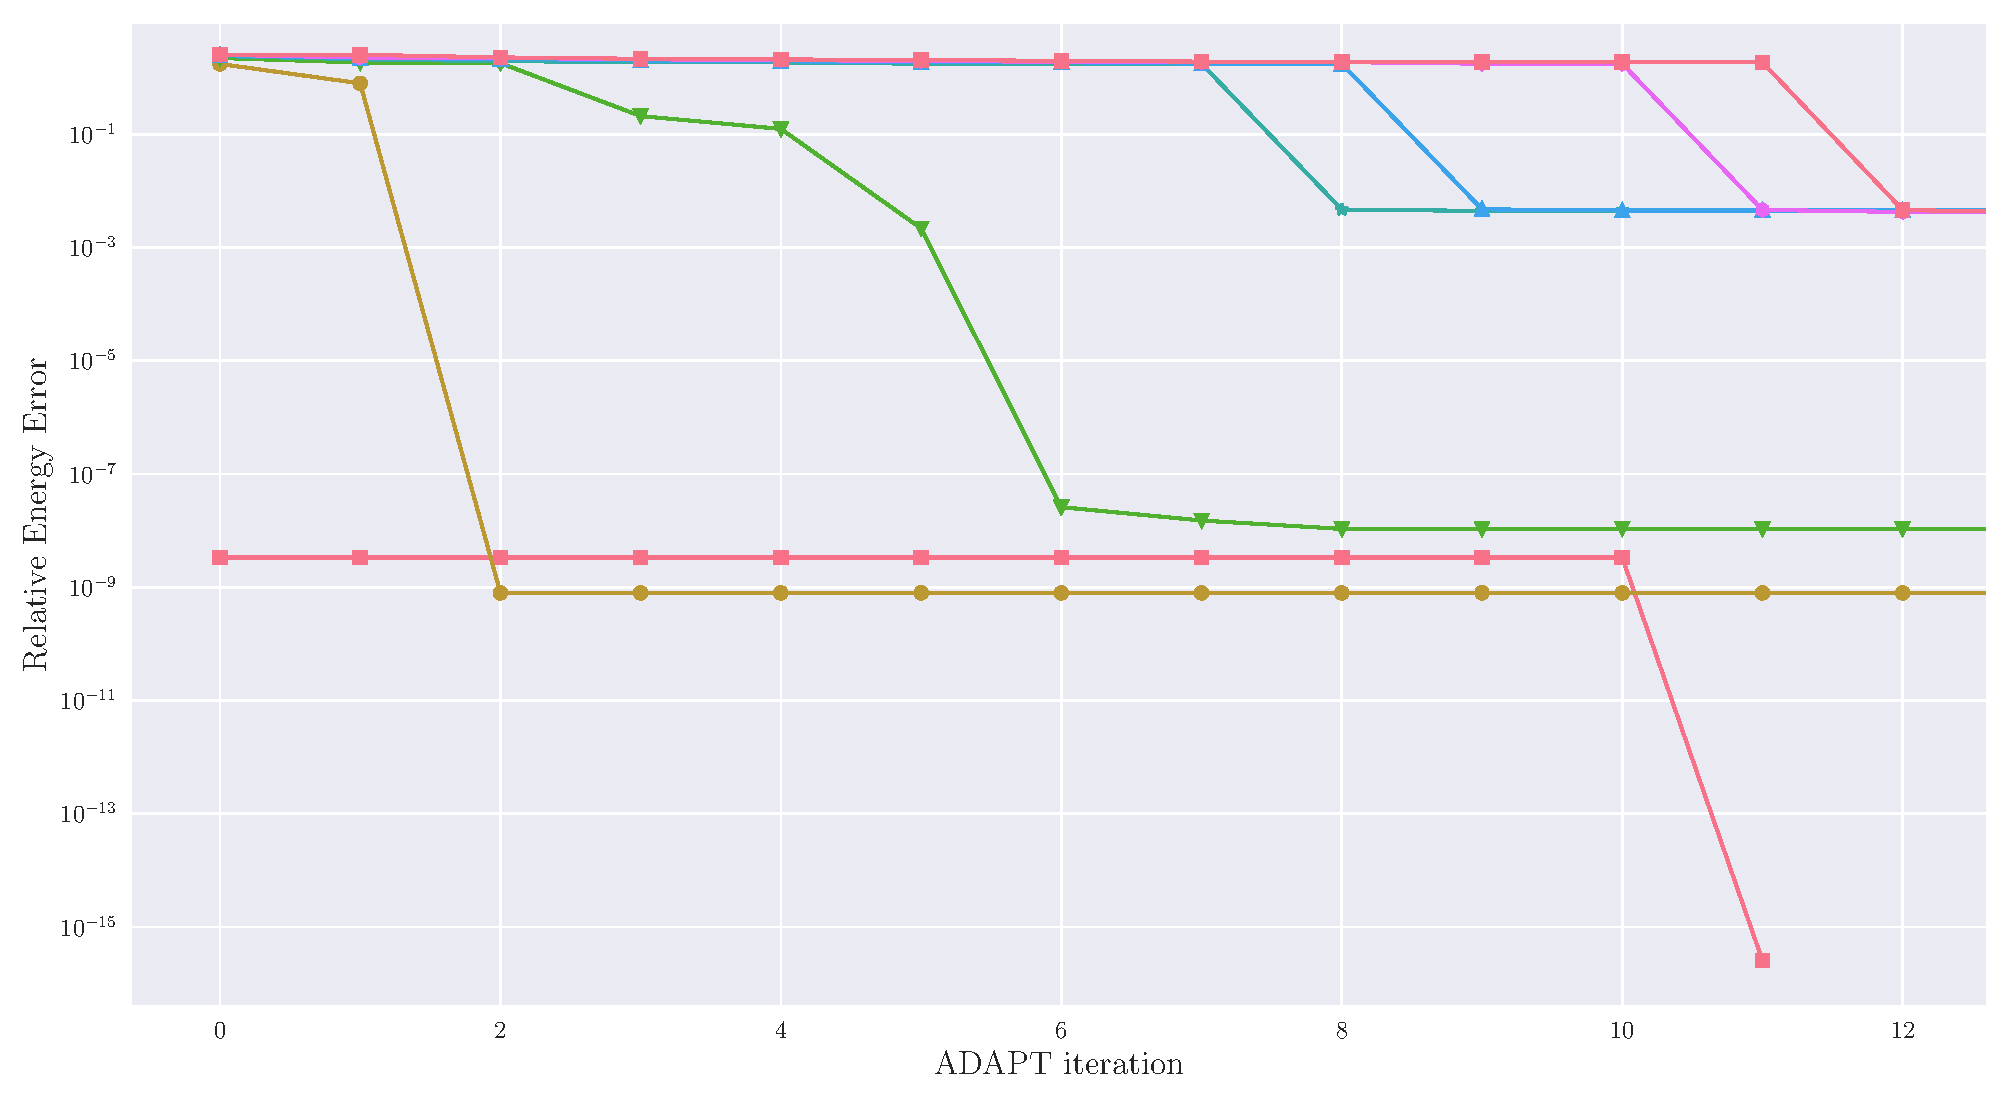
\includegraphics[width=0.7\linewidth]{image/deuteron_result/howmanyiters_zoomzoom.pdf}
    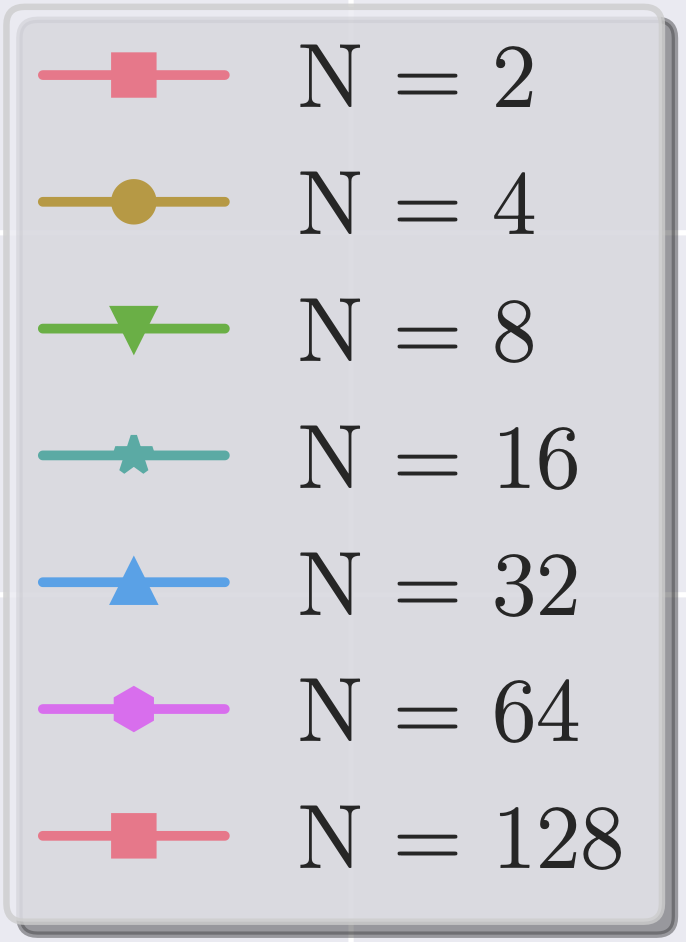
\includegraphics[width=0.2\linewidth]{image/legend.png}
\caption{Number of ADAPT iterations for the deuteron model with exact energy calculation optimised with \texttt{SLSQP}  for $ 1 $ to $ 7 $ qubits with maximum $ 100 $ iterations using the $ G $  pool. The pink line to the left with lower errors corresponds to the $ 1 $ qubit case, and the other pink line corresponds to $ N=128 $, the $ 7 $-qubit case. The top figure shows the whole $ 100 $ iteration, the middle figure shows a zoomed-in version of the top figure for around $ 27 $ iterations, and the bottom figure shows a zoomed-in version of the middle figure for around $ 13 $ iterations.}
    \label{fig:howmany}
\end{figure}

Finally, in an attempt to improve results further, we employed a new initialisation method, where the optimised state from the VQE is used as an initial state of the ADAPT-VQE. This is possible on actual hardware as well, since we know the structure of the ansatz and the optimal parameters. One could simply run the hardware efficient ansatz circuit with the optimal parameters before starting the ADAPT iterations.

\subsection{Initial States}
\label{sub:deuteron_initstate}
The initial state has a significant impact on the convergence of the ADAPT-VQE and VQEs in general. We have found that by utilising the HardwareEfficientAnsatz optimised state as the initial state, the ADAPT-VQE is able to converge to the correct state much faster, as shown in Figure~\ref{fig:whyoptinit}. When a small number of maximum iteration $ (5) $ is used, the ADAPT did not converge to the ground state for more than $ 2 $ qubits due to the limitation on iteration number. However, when the state was initialised with the hardware optimised state, the ADAPT-VQE with both pools converged to the minimum with error to orders of $ 10^{-2} $ or lower, even when the $ Ry $ state did not converge to the minimum. This could be extremely useful as it is usually not expensive in terms of both quantum and classical resources. This is similar to initialising it to the  HF state, except this way we could potentially start in an entangled state which the HF state often is not. We also do not rely on classical many-body methods, which should be preferable.

\begin{figure}[ht]
    \centering
    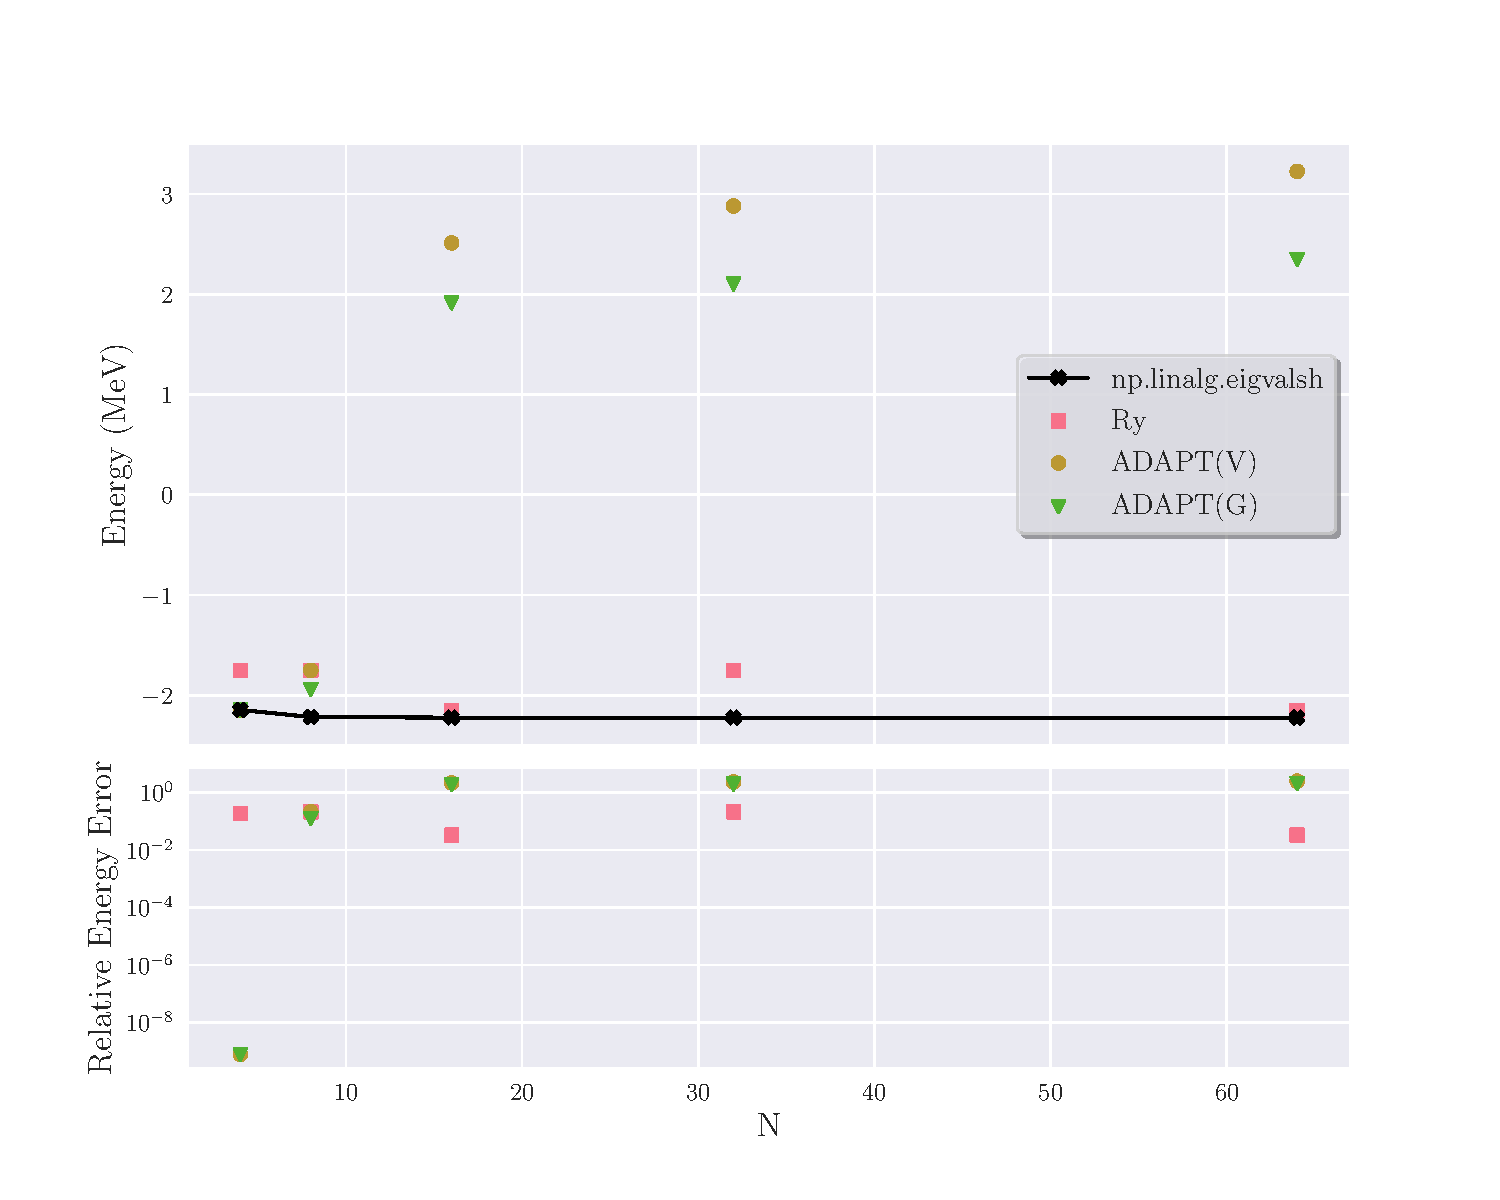
\includegraphics[width=0.8\linewidth]{image/deuteron_result/why_opt_init/S_NE_SLSQP_max_iter=5_hw_rep=2_(2,6,5)deutron_energies.pdf}
    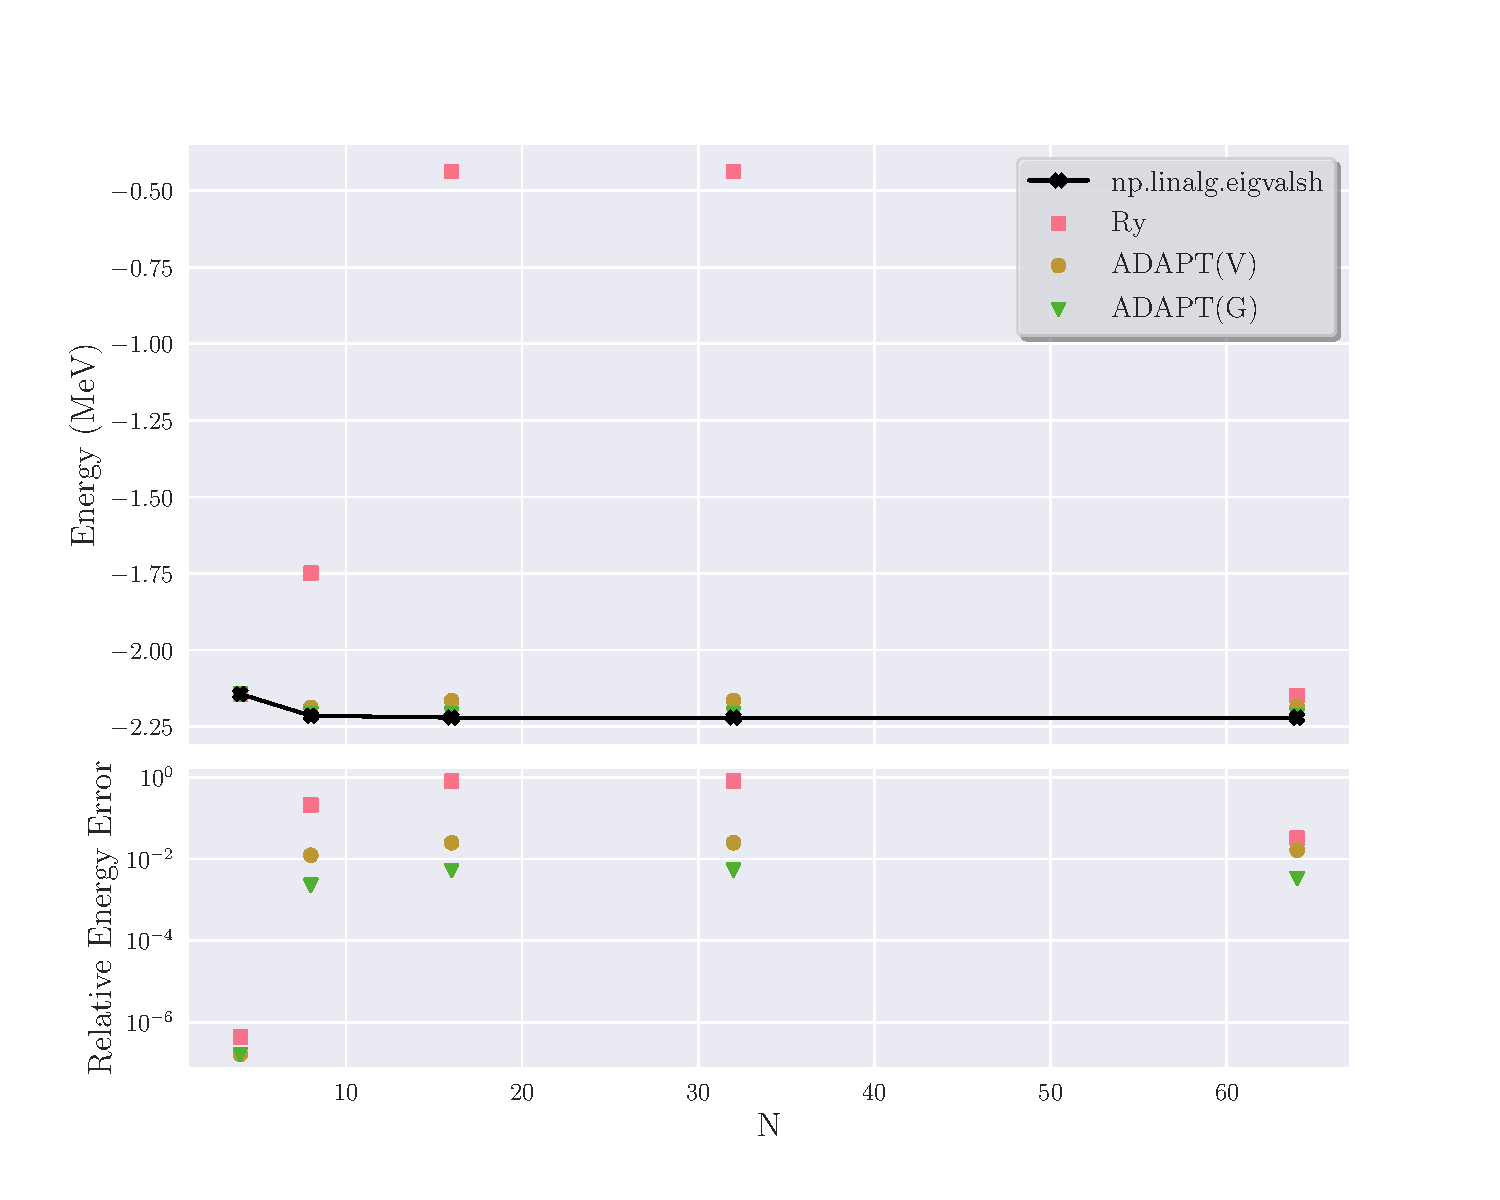
\includegraphics[width=0.8\linewidth]{image/deuteron_result/why_opt_init/S_NE_SLSQP_max_iter=5_hw_rep=2_opt_init_(2,6,5)deutron_energies.pdf}
    \caption{Results obtained for the deuteron Hamiltonian with different basis dimensions $ N $ with \textbf{exact energy calculation} for $ 5 $ maximum iterations and $ 2 $ repetition for the Hardware Efficient Ansatz Ry. The exponentials were decomposed using the \textbf{staircase} algorithm, and both VQEs were optimised with the \texttt{SLSQP} method. The top figure shows the results when the initial state is the maximally superposed state, and the bottom figure shows the results when the initial state is the Hardware Efficient Ansatz optimised state.}
    \label{fig:whyoptinit}
\end{figure}

